\documentclass[a4paper, 12pt, abstracton]{scrartcl}
\usepackage[utf8]{inputenc}     % keyboard import
\usepackage[UKenglish]{babel}   % keyboard english
\usepackage{siunitx}            % correct presentation of numbers and units
\usepackage{lmodern}            % other caracter type
\renewcommand{\familydefault}{\sfdefault} % man kann neue Befehle so definieren
%\newcommand{\unit}[1]{\ensuremath{\, \mathrm{#1}}}
\newcommand{\degree}{\ensuremath{^\circ}}
\usepackage{amssymb, amsmath, cancel, ulem, graphicx, float, tabularx, multirow, bm}
\usepackage{braket}     % Für QT
\usepackage{verbatim}
\usepackage{caption}
\usepackage{subcaption}
\usepackage{mathtools}
\usepackage{tablestyles}
\usepackage{enumitem}
\usepackage{tikz}
\usepackage{graphicx}
\usepackage{fixltx2e}	% Um Text tief zu stellen
\usepackage{booktabs}	% Tabellenformatierung
\usepackage{pdfpages}	% to include PDFs
\usepackage{listings}
\usepackage{color} %red, green, blue, yellow, cyan, magenta, black, white
\definecolor{mygreen}{RGB}{28,172,0} % color values Red, Green, Blue
\definecolor{mylilas}{RGB}{170,55,241} % ?
\usepackage{commath}
\usepackage{nameref}
\usepackage{wrapfig}
\usepackage{breakurl}
\usepackage{longtable}
\usepackage{url}
\usepackage{listings}
\usepackage[utf8]{inputenc} % Umlaute
\usepackage{hyperref}
\usepackage{chemist} % Für chemische Formeln noch anschauen!
\usepackage[noabbrev]{cleveref}
\newcommand{\sectionbreak}{\clearpage} % jedes Kapitel auf separate Seite starten
\renewcommand{\UrlFont}{\ttfamily\footnotesize} % font size url verkleinern

\usepackage[font=normalsize,labelfont=bf]{caption} % setzten der Schriftgrösse von caption
%\usepackage[font=scriptsize,labelfont=bf]{subcaption} % setzten der Schriftgrösse von subcaption

\DeclareCaptionFont{normalsize}{\normalsize\fontfamily{ptm}}
\captionsetup{textfont={normalsize}}

\usepackage{textgreek}
\usepackage{etoolbox}
\AtBeginEnvironment{tabular}{\normalsize\fontfamily{ptm}\selectfont} % Setzt Schriftart auf Times NewRoman

\setlength\parindent{0pt}
\setlength{\parskip}{6pt}

% For Bibliography
\usepackage[nottoc]{tocbibind}
\usepackage[square,numbers]{natbib}	% Für Biblio in Inhaltsverzeichnis ein
\bibliographystyle{abbrvnat}		% Typ wie Bibliography dargestellt wird.

\usepackage{times}					% Packet für Schriftart times

% Kopf-/Fusszeile
\usepackage{fancyhdr}   \pagestyle{fancy}
\lhead{} \chead{} \rhead{\leftmark}		% \leftmark = Name of the chapter
\lfoot{} \cfoot{\thepage}	% \thepage = page number at this position
\renewcommand\headrulewidth{2pt}
\renewcommand\footrulewidth{0.4pt}
\newcommand{\notes}[1]{{\color{red}{#1}}}
%\newcommand{\notes}[1]{} To delet all comments

	

\begin{document}
\renewcommand{\arraystretch}{1.5} % Macht Abstand der einzelnen Zeilen in einer Tabelle grösser
\fontfamily{ptm}\selectfont			% Setzt Schriftart auf Times NewRoman


\includepdf[pages={1-}]{Title_page.pdf}
\begin{comment}
	\begin{titlepage}
		
		\begin{flushright}
			\includegraphics[width=0.25\textwidth]{Bilder/logo-uni.jpg}\\[2cm]    
		\end{flushright}
		
		\begin{center} % Titelseite nach Unistandart einfügen ;)
			\huge \bfseries Calibration of the Neutral Gas and Ion Mass Spectrometer for the JUpiter ICy moons Explorer \\[2cm]
			\Large Inauguraldissertation der Philosophisch-naturwissenschaftlichen Fakultät der Universität Bern\\[1.5cm]
			\Large vorgelegt von\\[0.1cm]
			\Large Martina Föhn\\[0.8cm]
			\Large 2021\\[1cm] % Date of the Defence
			\Large Leiter der Arbeit\\[0.1cm]
			\Large Prof. Dr. Peter Wurz\\[1cm]
			\Large Physikalisches Institut der Universität Bern\\
			
		\end{center}
	\end{titlepage}
\end{comment}
	%------------------------------------------------------------------------------
	
	\newpage
	\thispagestyle{empty}
	\null
	\newpage
	\pagenumbering{roman}
	\begin{abstract}
		% Intro is ok. Somehow improve it to let it be more like advertising the thesis instead of a Praktikumsbericht...
		\noindent
		The JUpiter ICy moons Explorer (JUICE) of the European Space Agency (ESA) has the purpose to investigate Jupiter and his icy moons Europa, Ganymede and Callisto in great detail. JUICE will investigate the Jupiter system as a potential habitable system because the three icy moons have subsurface oceans where life might be possible. On board of JUICE is the Particle Environment Package (PEP), which consists of six individual instruments measuring electrons, ions and neutral particles in an energy range from meV up to MeV. One of these six instruments is the Neutral gas and Ion mass spectrometer (NIM). The NIM instrument is designed to measure the chemical and isotope composition of the icy moons' exospheres during the flybys of JUICE on the icy moons and also during JUICE final destination on Ganymede. The chemical and isotope composition allow a better understanding of the origin and evolution processes involved in the formation processes of the icy moons and our solar system.\\
		
		\noindent
		NIM is a time-of-flight mass spectrometer able to measure thermal neutral molecules and ionospheric ions. This thesis shows the journey from finalising the flight design of the NIM instrument to the actual testing and delivery of the NIM Proto-Flight (PFM) instrument in December 2020 to the JUICE spacecraft. On this journey, different flight components were tested and analysed as they came available during the development and finalization of the PFM and Flight-Spare (FS) instrument. From the foreseen scientific scope for the NIM instrument, a list of measurement requirements was delivered. This work shows that NIM PFM and NIM FS meet all these requirements.
		
	\end{abstract}

%----------------------------------------------------------------------------------
	\newpage
	\thispagestyle{empty}
	\null
	\newpage

	\tableofcontents

	\newpage
	\thispagestyle{empty}
	\null
	\newpage
	
	\section*{List of Acronyms}
		
	\begin{small}
	\begin{longtable}{>{\bfseries}m{2cm}|m{5cm}|>{\bfseries}m{2cm}|m{5cm}}
		ADC		& Analogue-to-Digital Converter & NIM & Neutral Gas and Ion Mass Spectrometer \\
		CASYMIR	& CAlibration SYstem for the Mass spectrometer In\-stru\-ment ROSINA & NIMS	& Near Infrared Mapping Spectrometer\\
		CReMA	& Consolidated Report on Mission Analysis & NGMS & Neutral Gas Mass Spectrometer \\
		ESA		& European Space Agency & P-BACE	& Polar Balloon Atmospheric Composition Experiment \\
		Fil		& Filament electrode & PCB		& Printed Circuit Board \\
		FoV		& Field-of-View & PEP   	& Particle Environment Package \\
		FS		& Flight-Spare Model & PFM		& Proto-Flight Model \\
		FWHM  	& Full Width at Half Maximum & R		& Reflectron (ion-mirror) \\ 
		HV		& High-Voltage & ROSINA	& Rosetta Orbiter Spectrometer for Ion and Neutral Analysis\\
		i		& ion & RTG		& Radioisotope Thermoelectric Generators\\
		IS		& Ion-Source & RTOF	& Reflectron Time-Of-Flight mass spectrometer\\
		JDC		& Jovian plasma Dynamics and Composition analyser & S/C		& Spacecraft \\
		JEI		& Jovian Electrons and Ions & SATANS	& Supersonic cATion and ANion Source \\
		JENI	& Jovian Energetic Neutrals and Ions & SN		& Serial Number \\
		JNA		& Jovian Neutrals Analyser & SNR		& Signal-to-Noise Ratio \\
		JoEE	& Jovian Energetic Electrons & 	TF		& Time Focus \\
		JUICE 	& JUpiter ICy moon Explorer & th		& thermal \\ 
		LV 		& Low-Voltage & TOF		& Time-Of-Flight \\
		MCP		& Multi-Channel-Plate & &\\
		MEAP	& Mars Environment Analogue Platform & & \\
		n		& neutral & & \\
	\end{longtable}
	\end{small}
	\newpage
	\thispagestyle{empty}
	\null
	\newpage
	
	\pagenumbering{arabic}

	% !TEX root = arbeit.tex
% Damit Latex weiss, wo die main Datei ist.
\section{Introduction}

	\subsection{Mission}
	Motivation to fly to Jupiter and his Icy moons. Mission explanation with an explanation why TOFs are used and better than other types of sensors to analyse the moons exospheres (Refs. to Audrey, Salome...).\\
	If there is an explanation where TOFs were used so far, than its in this chapter. In the next there is only technical staff about TOFs. For references see Paper and Rico's diss.\\
	JUICE PEP NIM
	
	\subsection{Requirements}
	Mass, performance, Power consumption. (See latest references. Part of the introduction?)
	Either give a short overview with references to the different subchapters in the Disseration as a guideline. At that point, the people don't know anything about the instrument.
	
	\subsection{Diss Overview} % is currently the start of the theory part.
	Scope of the thesis. Give a short overview over the chapter to explain that in the theory part the different compartments are analysed from the theoretical point of view and in the experimental part, there are made tests of the different compartments. Does it make sense to do it so if there is not explained how the spectrometer works? Only stat it on a very rudimentary level.	
	
	% Rico's Diss
	\begin{comment}
	Planetology depends on simulations but there are also instruments needed to verify the models and set constrains for them. Optical techniques as ultraviolet (UV), visible (VIS), infrared (IR) spectroscopy. On space craft or on earth such as ALMA...
	laser ionization mass spectroscopy (LIMS) for lander to analyse the soil.
	Mass spectrometry has better sensitivity because there single atoms are counted 
	
	\end{comment}
		
	\begin{comment}
		Why a TOF compared to other types of mass spectrometers such as sector magnets or quadrupols.Costumisatoin to the needs of the of the mission (GC for NGMS).
		Improvement in the electronics.
	\end{comment}
	
	
	
	
	
	
	
	
	
	
	
	
	
	
	
	
	\newpage
	\thispagestyle{empty}
	\null
	\newpage
	% !TEX root = arbeit.tex
\section{Theory} % Rearrange the figures before sending
% Short overview with references to the different chapters which analyse certan parts a bit more in detail. Part of the Intro? Can still be move into the intro part.
	% Ionisation efficiency, Time focusing, SNR definition, Sensitivity estimation. Nessesary? If so, part of SNR discussion. Not used in the experiments explained so far...	
	\notes{Rewrite} NIM is a time-of-flight mass spectrometer consisting of an ion-source, a mass analyser and a detector. Particles enter the ion-source either through a closed source antechamber where they get thermalized or directly through an entrance slit. When particles enter through the antechamber, the measuring mode is called th-mode. When neutral particles enter through the entrance slit, the mode is called n-mode and when the ions enter the slit, the mode is called i-mode. The neutral particles get ionized by electron ionization. All ions are accelerated by applying a high voltage pulse on the extraction grid to the same energy. Light species fly faster through the spectrometer than heavier ones resulting in a separation of the species by their mass. An ion-mirror is used to increase the flight distance and to refocus ions of the same species with different energies. % Write it a bit better.
	The ions are detected with a Multi-Channel-Plate (MCP) detector.\\
	This chapter gives an overview from the theoretical perspective over the different subunits of NIM where in chapter \notes{Ref: Exp.} the different subunits are tested.
	\begin{figure}[h]
		\centering
		\includegraphics[width= 10cm]{Bilder/NIM_Sketch.png}
		\caption{Schematics of the NIM mass spectrometer. Adapted from \cite{Diss_Meyer}.}
		\label{fig:NIMSketch}
	\end{figure}
	% Give here sort of an outlook to the different chapters after the overview of the instrument.
	
	
	%------------------------------------------------------------------------------------------------
	\subsection{Mass Resolution \notes{finished}}\label{chap:massRes}
	The generated ions in the ion-source are focused in the centre and extracted by a high voltage pulse applied onto the extraction grid. All ions are accelerated to the same energy $W$:
	\begin{equation}
		W = \int_{0}^{s_0}q E_s ds =  \frac{q U_0}{2}
		\label{eq:WIonPulse}
	\end{equation}
	With $s_0$ the distance from the centre of the ion-source to the extraction grid corresponding to half the height of the ion-source. $q$ is the particle charge, $E_s$ is the applied electric field strength induced by the voltage $U_0$ applied on the extraction grid. The ions start in the centre of the ion-source. Therefore, they have the kinetic energy $q U_0/2$ when reaching the extraction grid:
	\begin{equation}
		\frac{q U_0}{2} = \frac{1}{2}m v^2
	\end{equation}
	With $m$ and $v$ the mass and velocity of the ion. Rearranging this formula results in:
	\begin{equation}
		\frac{m}{q} = U_0\frac{t^2}{D^2}
		\label{eq:m/q}
	\end{equation}
	With $t$ the time of flight and $D$ the flight distance from the extraction grid to the detector. $U_0$ and $D^2$ are merged into one constant $C$ resulting in:
	\begin{equation}
		\frac{m}{q} = C(t-t_0)^2
		\label{eq:mass_Calib}
	\end{equation}
	$t_0$ corresponds to a time offset between the start of the mass axis and the time axis. The two calibration constants $C$ and $t_0$ are determined by at least knowing two species in the spectrum. The mass is therefore proportional to $t^2$:
	\begin{equation}
		m = c\cdot t^2
		\label{eq:mt2}
	\end{equation}
	The derivative is:
	\begin{align}
		\frac{dm}{dt} &= 2~ct\\
		dm &= 2~ct\cdot dt
		\label{eq:dm}
	\end{align}
	Dividing Eq.\,\eqref{eq:mt2} through Eq.\,\eqref{eq:dm} results in:
	\begin{align}
		\frac{m}{dm} &= \frac{ct^2}{2~ct\cdot dt}\\
		\frac{m}{dm} &= \frac{t}{2~dt} = \frac{\mu}{2\cdot FWHM}
		\label{eq:massRes}
	\end{align}
	With $\mu$ the centre of the mass peak in the time domain and $FWHM$ is the full width at half maximum of the mass peak \cite{LecNot_Wurz2017}.\\
	
	In the following section, the different contributions affecting the mass resolution are analysed. The focus is on the contributions originating from the source thus they have the biggest impact on the mass resolution of the instrument.\\
	The total time spread $dt_i$ of the signal of a particle species $i$ is:
	\begin{equation}
		dt_i = \sqrt{\sum_{k} dt_k^2} = \sqrt{dt_D^2 + dt_{ADC}^2 + dt_{th}^2 + dt_{s}^2 + dt_{tfall}^2} 
	\end{equation}
	With the different contributions $dt_k$. When an ion hits the detector, it generates a voltage pulse with pulse width $dt_D$. For the NIM detector, the pulse width is $\sim$~0.7~ns. The generated pulse is converted into a digital signal with an analog-to-digital converter (ADC). The ADC used in the laboratory has a sampling rate of 4~GHz resulting in a time resolution $dt_{ADC}$ of 0.25~ns. The flight ADC has a maximal sampling rate of 2~GHz corresponding to a time resolution of 0.5~ns.\\
	\begin{figure}[h] % space and velocity deviation.
		\centering
		
\includegraphics[width= \textwidth]{Bilder/ISStartPosThermEn.png}
		\caption{Flight path of ions with different thermal energy (top panel) and start positions (lower panel). $v_{init}$ is the initial velocity of the ions and $dt_{th}$ the turn-around time.}
		\label{fig:thISStartPosThermEn}
	\end{figure}
	\begin{figure}[h!]
		\begin{subfigure}{0.5\textwidth}
			\centering
			\includegraphics[width=\textwidth]{Bilder/PulserShapeTheoAna.png}
			\caption{}
			\label{subfig:theoPulseShape}
		\end{subfigure}
		\begin{subfigure}{0.5\textwidth}
			\centering
			\includegraphics[width=.9\textwidth]{Bilder/PulserFallTimeShapes.png}
			\caption{}
			\label{subfig.PulserFallTimeShapes}
		\end{subfigure}
		\caption{a) Shape of a realistic high voltage pulse applied on the extraction grid. b) Two different possible shapes of the falling edge of the high voltage pulse.}
		\label{fig:theoPulseShape}
	\end{figure}
	\begin{figure}[h] % Electric field vs. position s
		\centering
		\includegraphics[width= 0.7\textwidth]{Bilder/PulsInt.png}
		\caption{Top panel: Electric field $E(s)$ an ion experiences, as a function of the distance between the centre of the ionisation region and the extraction grid $s_0$ for two hydrogen (H\textsubscript{1}) and oxygen (O\textsubscript{1}). $s_i(t_{fall})$ is the position of the corresponding species at the fall time $t_{fall}$. Lower panel: Energy $W(s)$ of the ions as a function of their position.}
		\label{fig:PulsInt}
	\end{figure}

	The time spreads resulting from the thermal energy of the ions $dt_{th}$, from the different start positions of the ions within the ionisation region $dt_s$ and from the fall time of the high voltage pulse $dt_{tfall}$ are coupled because they all affect the energy deviation of the ions.
	The ions in the ion-source have thermal energy $W_{th}$:
	\begin{equation}
		W_{th} = \frac{3}{2}\cdot k_B \cdot T
	\end{equation}
	With $k_B$ the Boltzmann constant and $T$ the temperature. The thermal energy leads to an initial velocity of the ions $v_{init}$ (Fig.\,\ref{fig:thISStartPosThermEn} top panel). Ions number 1 and 3 have the same thermal energy but one points towards the extraction grid where the other one points towards the backplane. When a high voltage pulse is applied on the extraction grid, ion number 3 has to be turned around. The time offset between ions 1 and 3 is called turn-around time. At a certain point in time, ion 3 will overtake ions with less energy (ion 1). The turn-around time cannot be corrected with the ion optics. The only option to reduce the turn-around time would be to cool the ions, which is not possible for a space instrument.\\
	The total energy $W$ the ions get in the ionisation region is:
	\begin{equation}
		W = \int_{s_{init}}^{s_0} q\cdot E(t)\cdot ds
		\label{eq:WionsISposEt}
	\end{equation}
	With $s_{init}$ the initial position of the ions, $s_0$ the distance from the centre of the ionisation region to the acceleration grid, $q$ the particle charge and $E(t)$ the electric field strength depending on the time $t$. When the ions start at different positions in the ionisation region $s_{init}$, they receive a different amount of energy because they travel a different distances in the acceleration field (Fig.\,\ref{fig:thISStartPosThermEn} lower panel). Ions, which are closer at the backplane receive more energy but start later at the extraction grid than ions, which start closer at the extraction grid. At a certain distance, the ions with higher energy will overtake the other ions. The time deviation induced by the different start positions of the ions is $dt_{s}$. With an ion-mirror ions with an energy deviation up to 10\% are refocused. Ions with higher energy penetrate deeper into the ion-mirror resulting in a longer flight path of the higher energetic ions. The best position for the detector is when all ions with different energies are at the same position.\\
	% This point is at around $2\cdot s_0$ which corresponds to a very short flight distance. To shift this focal point onto to the detector, additional electric fields are applied right after the extraction grid in the ion-source to move the focal spot onto the detector.\\
	Ideally, the shape of the extraction pulse is a rectangle. Fig.\,\ref{subfig:theoPulseShape}) shows the shape of a realistic extraction pulse. The pulse needs the time $t_{fall}$ to build up on the extraction grid. Fig.\,\ref{fig:PulsInt}~top shows the changing electric field as a function of the position for atomar hydrogen (H\textsubscript{1}) and oxygen (O\textsubscript{1}) in case when these two species start at the same position. The total energy $W$ of the ions corresponds to the area under the curves. The energy as a function of the flight distance $s$ in the ionisation region and is plotted on the bottom panel of Fig.\,\ref{fig:PulsInt}. Hydrogen is lighter than oxygen and therefore, it leaves the ionisation region earlier. This results in a smaller amount of energy for hydrogen than for oxygen. The shorter the fall time of the high~voltage pulse is, the smaller is the energy difference because it shifts the position of the ions at the fall time $s_i(t_{fall})$ towards zero. When looking at the shape of the falling edge of the pulse (Fig.\,\ref{subfig.PulserFallTimeShapes}), it is more important to have a small fall time with an overshoot than a pulse slowly converging to the maximum because the resulting energy deviation in the first case is much smaller than in the second.\\
	
	In the following section the influence of the fall time of the high~voltage pulse $t_{fall}$ in combination with the spacial deviation $\Delta s$ and the thermal energy of the ions on the mass resolution is analysed. To investigate the impact of these effects, this model does not include any focusing lenses and has no ion-mirror.\\
	The derivation of the equation of motion is based on \cite{Diss_Abplanalp}. The electric field $E(t)$ in the ionisation region is approximated with a linear function during the fall time $t_{fall}$ and as a constant during the rest of the time:
	\begin{equation}
		E(t) =
		\begin{cases}
			E_1\cdot\frac{t}{t_{fall}},& (0\leq t\leq t_{fall})\\
			E_1,& t_{fall} < t
		\end{cases}
	\label{eq:PulseEt}
	\end{equation}
	$E_1$ is the electric field strength when the high voltage pulse is fully applied:
	\begin{equation}
		E_1 = \frac{U_0}{2\cdot s_0}
	\end{equation}
	With $U_0$ the voltage on the extraction grid. The equation of motion for the ions during the fall time is:
	\begin{equation}
		a_{fall}(t\leq t_{fall}) = \frac{q\cdot E_1}{m\cdot t_{fall}}\cdot t
		\label{eq:afall}
	\end{equation}
	With $a_{fall}$ the acceleration of the ions and $m$ the ion mass. The velocity of the ions $v_{fall}$ is:
	\begin{equation}
		v_{fall}(t\leq t_{fall}) = \frac{q\cdot E_1}{2\cdot m\cdot t_{fall}}\cdot t^2 + v_{init}\label{eq:vfall}
	\end{equation}
	With $v_{init}$ the initial velocity of the ions before applying the extraction pulse. The position of the ions $s_{fall}$ at the time $t$ is:
	\begin{equation}
		s_{fall}(t\leq t_{fall}) = \frac{q\cdot E_1}{6\cdot m\cdot t_{fall}}\cdot t^3 + v_{init}\cdot t + s_{init}
		\label{eq:sfall}
	\end{equation}
	With $s_{init}$ the initial position of the ions. When the high voltage pulse is fully applied and the ions did not reach the extraction grid until that time, the acceleration of the ions $a_{p}$ is:
	\begin{equation}
		a_{p}(t > t_{fall}) = \frac{q\cdot E_1}{m}
		\label{eq:ap}
	\end{equation}
	The velocity $v_{p}$ is:
	\begin{equation}
		v_{p}(t > t_{fall}) = \frac{q\cdot E_1}{m}(t-t_{fall}) + v_{fall}(t_{fall})
		\label{eq:vp}
	\end{equation}
	With $v_{fall}(t_{fall})$ the velocity of the ions at the time $t_{fall}$. The position $s_{p}$ is:
	\begin{equation}
		s_{p}(t > t_{fall}) = \frac{q\cdot E_1}{2\cdot m}(t-t_{fall})^2 + v_{fall}(t_{fall})(t-t_{fall}) + s_{fall}(t_{fall})
		\label{eq:sp}
	\end{equation}
	With $s_{fall}(t_{fall})$ the position of the ions at the time $s_{fall}$. When the ions leave the ionisation region before full high voltage is applied on the extraction grid, the time they spend in the ionisation region $t_{IS}$ is calculated by setting $s_{fall}=s_0$ and solving the cubic Eq.\,\eqref{eq:sfall} to $t$. The velocity $v_{Grid}$ of the ions at the extraction grid is determined by inserting $t_{IS}$ in Eq.\,\eqref{eq:vfall}.\\
	When the ions leave the ionisation region after the high voltage is fully applied, the time they spend in the ionisation region $t_{IS}$ is calculated by setting $s_{p}=s_0$ and solving Eq.\,\eqref{eq:sp} to $t$. The velocity $v_{Grid}$ of the ions at the extraction grid is determined by inserting $t_{IS}$ in Eq.\,\eqref{eq:vp}. The total flight time of the ions in this model is:
	\begin{equation}
		t_{TOF} = t_{IS} + t_D
	\end{equation}
	With $t_{D}$ the time of flight the ions need for the distance between the extraction grid and the detector. The mass resolution is calculated according to Eq.\,\eqref{eq:massRes}. To have a measure for the impact of the fall time on the different masses, the deviation $R$ of the mass resolution of ions with a mass/charge ratio $i$ relative to the mass resolution of ions with a mass/charge ratio of 200 is calculated:
	\begin{equation}
		R = 1 - \frac{m_i/\Delta m_i}{m_{200}/\Delta m_{200}}
	\end{equation}
	The mass resolution reaches a plateau for high mass particles (cf. Fig.\,\ref{fig:Simtfall}~left). The deviation $R$ is a measure by how many percent the mass resolution of the low mass particles deviates from that plateau. The mass resolution of mass/charge ratio 200 was taken as a reference.\\
	\begin{figure}[h] % Fall time plots
		\centering
		\includegraphics[width=\textwidth]{Bilder/PulseSimMassRes.png}
		\caption{Left: Simulated mass resolution as a function of the mass/charge ratio of the particles for three different pulser fall times. Right: relative deviation of the mass resolution from the plateau as a function of the mass/charge ratio.}
		\label{fig:Simtfall}
	\end{figure}
	\begin{figure}[h!] % Lab WLE measurement
		\centering
		\includegraphics[width=.8\textwidth]{Bilder/PulseLabWLEm480.png}
		\caption{Measurement results of two different pulser generators with 1.5 ns and 3.5 ns fall time.}
		\label{fig:LabWLE}
	\end{figure}
	\begin{figure}[h!] % spatial deviation plots
		\centering
		\includegraphics[width=\textwidth]{Bilder/PulseSimPosition.png}
		\caption{Left: Simulated mass resolution as a function of the spacial deviation $\Delta s$ for three different pulser fall times. Right: relative deviation of the mass resolution from the plateau as a function of the mass/charge ratio.}
		\label{fig:SimtfallPos}
	\end{figure}
	The simulations revealed that the impact of the particle temperature is negligible compared to the impact of the position deviation $\Delta s$ and the pulse fall time $t_{fall}$. The impact of $t_{fall}$ is shown in Fig.\,\ref{fig:Simtfall} left. The position deviation is $\pm$~0.4~mm which corresponds to the diameter of the electron beam in the ionization region. With decreasing fall time, the deviation in mass resolution decreases. This is also visible in the right figure. An improvement in the fall time by one decade results in an improvement of 1~decade of the relative error. With a fall time of 1~ns, the maximum relative deviation is only 0.1~\%. The impact of the fall time is also visible in measurements. Fig.\,\ref{fig:LabWLE} shows measurements with two different pulse generators with fall times 1.5~ns and 3.5~ns.\\
	Fig.\,\ref{fig:SimtfallPos}~left shows the mass resolution as a function of the position deviation $\Delta s$ for mass 1~u. The ionisation region has a diameter of 2~mm. Therefore the maximal deviation of the ions is 1~mm. With increasing $\Delta s$ the mass resolution drops very rapidly. Therefore it is very important to focus the ions in the centre of the ionisation region. The better the ions are focused, the better is the mass resolution. The relative deviation increases significantly for position deviations close to 1~mm because there, some ions leave the source when the high voltage pulse is not fully applied.\\

%--------------------------------------------------------------------------------------------------	
	\subsection{Signal-to-Noise Ratio and Sensitivity \notes{Draft}}
	
	\textbf{SNR}\\ % Write a bit more detailed. What does background corrected mean? Subtraction of the baseline if it is elevated.
	The SNR is defined as the ratio of the background corrected peak amplitude $I^{max}_P$ and the standard deviation of the base line $std(I_b)$ \cite{Agilent_TechNote_SNR}, \cite{Master_Meyer}: % Thechnical Note Agilent and Masterarbeit Stefan.
	\begin{equation}
		SNR = \frac{I^{max}_P}{std(I_b)}
		\label{eq:SNR}
	\end{equation}
	A high mass resolution improves also the signal-to-noise ratio. By better focusing the ions in the time frame, the peak gets narrower. The area under the peak corresponds to the number of ions. If the number of ions and therefore the area under the curve stays the same, a narrower peak implicates an increase in signal height and therefore in a higher SNR.\\ % In other mass spectrometers (such as sector magnets) an increase in mass resolution results in a reduction of the phase space and therefore in a loss of signal intensity.
	\\
	\textbf{Sensitivity} \\ % Really include this chapter? Because it is only an estimation of the actual performance of the instrument. If it is included, do a proper derivation of the formula!!
	The sensitivity $n_{lim}$ is the actual detection limit of the sensor. It is defined as the amount of gas detected by the instrument $n_{det}$ over the amount of ions entering the instrument $n_{p}$ times the signal intensity measured by the instrument $I_{sig}$
	\begin{equation}
		n_{lim} = \frac{n_p \cdot I_{sig}}{n_{det}}
	\end{equation}
	
	
	\begin{comment}
		SNR
		[Wells 2011]
	\end{comment}
	
	\subsection{Ion Optical Design, NIM specific elements \notes{see Subchapters}} % Inspiration from the arguments of the paper. Titel noch anpassen. Ion source efficienies, reflectron double focusing, detector reflection of signal, signal matching.
	This section gives a detailed overview over the different subcomponents of NIM. Here, the fundamental theory parts for the NIM specific elements are explained. These elements are the functionality of the closed source antechamber, the shutter motor,...
	Later on in chapter \notes{Ref.} test results of the different components are shown.
	
	
		\subsubsection{Filament Power Calculation \notes{Draft}}
		% Also mention the importance of the filament position or does it make more sense if this whole part is in the Experiment part, thus there is only an phenomenological description of the behaviour?
		% Record also of the heating current. It strongly depends on the voltage set. But maybe we see a tendency of the behaviour over time with the uncertainty factor of the voltage set. -> have a look at the data.
		
		\subsubsection{Ion Storage \notes{finished}}\label{chap:IonStor}
		Ion storage of positive ions in the ionisation region is mainly achieved by the negative potential of the electron beam. Together with the other focusing electrodes in the ionization region, a trapping field is generated to store the ions during the time when no high-voltage pulse is applied on the extraction grid. Ion storage is important because every ion generated and not stored is lost. In addition, these ions add to the random noise level. In the following section, the potential in the centre of the electron beam is calculated. The electron emission current $I_{e}$ is:
		\begin{equation}
			I_{e} = n_e q_0 v\pi R_e^2
			\label{eq:theoElIem}
		\end{equation}
		With $n_e$ the electron volume density, $q_0$ the elementary charge, $v$ the velocity of the electrons and $R_e$ the radius of the electron beam (Fig.\ref{fig:thAntIs}). The electrons get accelerated by the negative potential applied at the filament base. This potential is -70\,\si{\volt} resulting in a kinetic energy $U$ of 70\,\si{\electronvolt}. The velocity of the electrons is:
		\begin{equation}
			v = \sqrt{\frac{2 U}{m_e}}
			\label{eq:theoElIemVelo}
		\end{equation}
		With $m_e$ the mass of the electron. Solving Eq.\,\eqref{eq:theoElIem} for the volume density $n_e$ and inserting Eq.\,\eqref{eq:theoElIemVelo} for the velocity results in:
		\begin{equation}
			n_e = \frac{I_e}{q_0 \pi R_e^2}\sqrt{\frac{m_e}{2U}}						\label{eq:theoElIemNe}
		\end{equation}
		The electric field $E(r)$ in the ionization region is calculated for $R_e<r<h_{Is}/2$ with $r$ the distance from the centre of the beam and $h_{Is}$ the height of the ion source. The electric flux is defined as the surface integral of the electric field through the surface of an enclosed volume which is in this case a cylinder volume. Using Gauss's law the electric flux through the beam surface $A_{beam}$ is equal to the total charge $Q$ inside the cylinder volume:
		\begin{align}
			A_{beam} E(r) &= \frac{Q}{\epsilon_0}\\
			2\pi r l E(r) &= \pi R_e^2 l n_e q_0 \frac{1}{\epsilon_0}
		\end{align}
		With $l$ the cylinder length, $q_0$ the elementary charge and $\epsilon_0$ the vacuum permittivity. Replacing the number density $n_e$ with Eq.\,\eqref{eq:theoElIemNe} and solving the equation for the electric field $E(r)$ results in:
		\begin{equation}
			E(r) = \frac{I_e}{2 \pi \epsilon_0} \sqrt{\frac{m_e}{2U}}\frac{1}{r}
		\end{equation}
		The potential $\Phi_o (r)$ at a position $r$ outside of the electron beam is:
		\begin{equation}
			\Phi_o (r) = -\int_{h_{Is}/2}^{r} E(r') dr' = -\frac{I_e}{2\pi\epsilon_0}\sqrt{\frac{m_e}{2U}}\ln\left(\frac{r}{h_{Is}/2}\right)
		\end{equation}
		The electric field inside the electron beam at position $0<r<R_e$ is calculated by using Gauss's law:
		\begin{equation}
			2\pi r l E(r) = \pi r^2 l n_e q_0 \frac{1}{\epsilon_0}
		\end{equation}
		Replacing the number density $n_e$ with Eq.\,\eqref{eq:theoElIemNe} and solving the equation for the electric field $E(r)$ results in:
		\begin{equation}
			E(r) = \frac{I_e}{2\pi\epsilon_0}\sqrt{\frac{m_e}{2U}}\frac{r}{R_e^2}
		\end{equation}
		The electric potential $\Phi_i (r)$ is:
		\begin{equation}
			\Phi_i (r) = -\int_{R_e}^{r} E(r') dr' = -\frac{I_e}{4\pi\epsilon_0}\sqrt{\frac{m_e}{2U}}\left(\frac{r^2}{R_e^2} -1 \right)
		\end{equation}
		And relative to border of the ion source:
		\begin{equation}
			\Phi_i (r) = -\frac{I_e}{4\pi\epsilon_0}\sqrt{\frac{m_e}{2U}}\left(2\ln\left(\frac{R_e}{h_{Is}/2}\right) +\frac{r^2}{R_e^2} -1 \right)
			\label{eq:elPotIem}
		\end{equation}
		For an electron emission current of 100~\si{\micro\ampere} the electric potential inside the electron beam is 0.75\,\si{\volt}. This potential is strong enough to trap light species such as water. For heavier species, NIM has a special designed ionisation region (Fig.\,\ref{fig:ISZoom}). The electrodes $IS 1$, $IS 5$ and $IS 6$ trap the ions in x-direction where the two ring electrodes $IS 2$ and $IS 4$ trap the ions in the other two directions.		
		\begin{figure}[h]
			\centering
			\includegraphics[width= .5\textwidth]{Bilder/NIM_schema_zoom_IS.png}
			\caption{Zoom of NIM's ionisation region.}
			\label{fig:ISZoom}
		\end{figure}
		\begin{figure}[h]
			\centering
			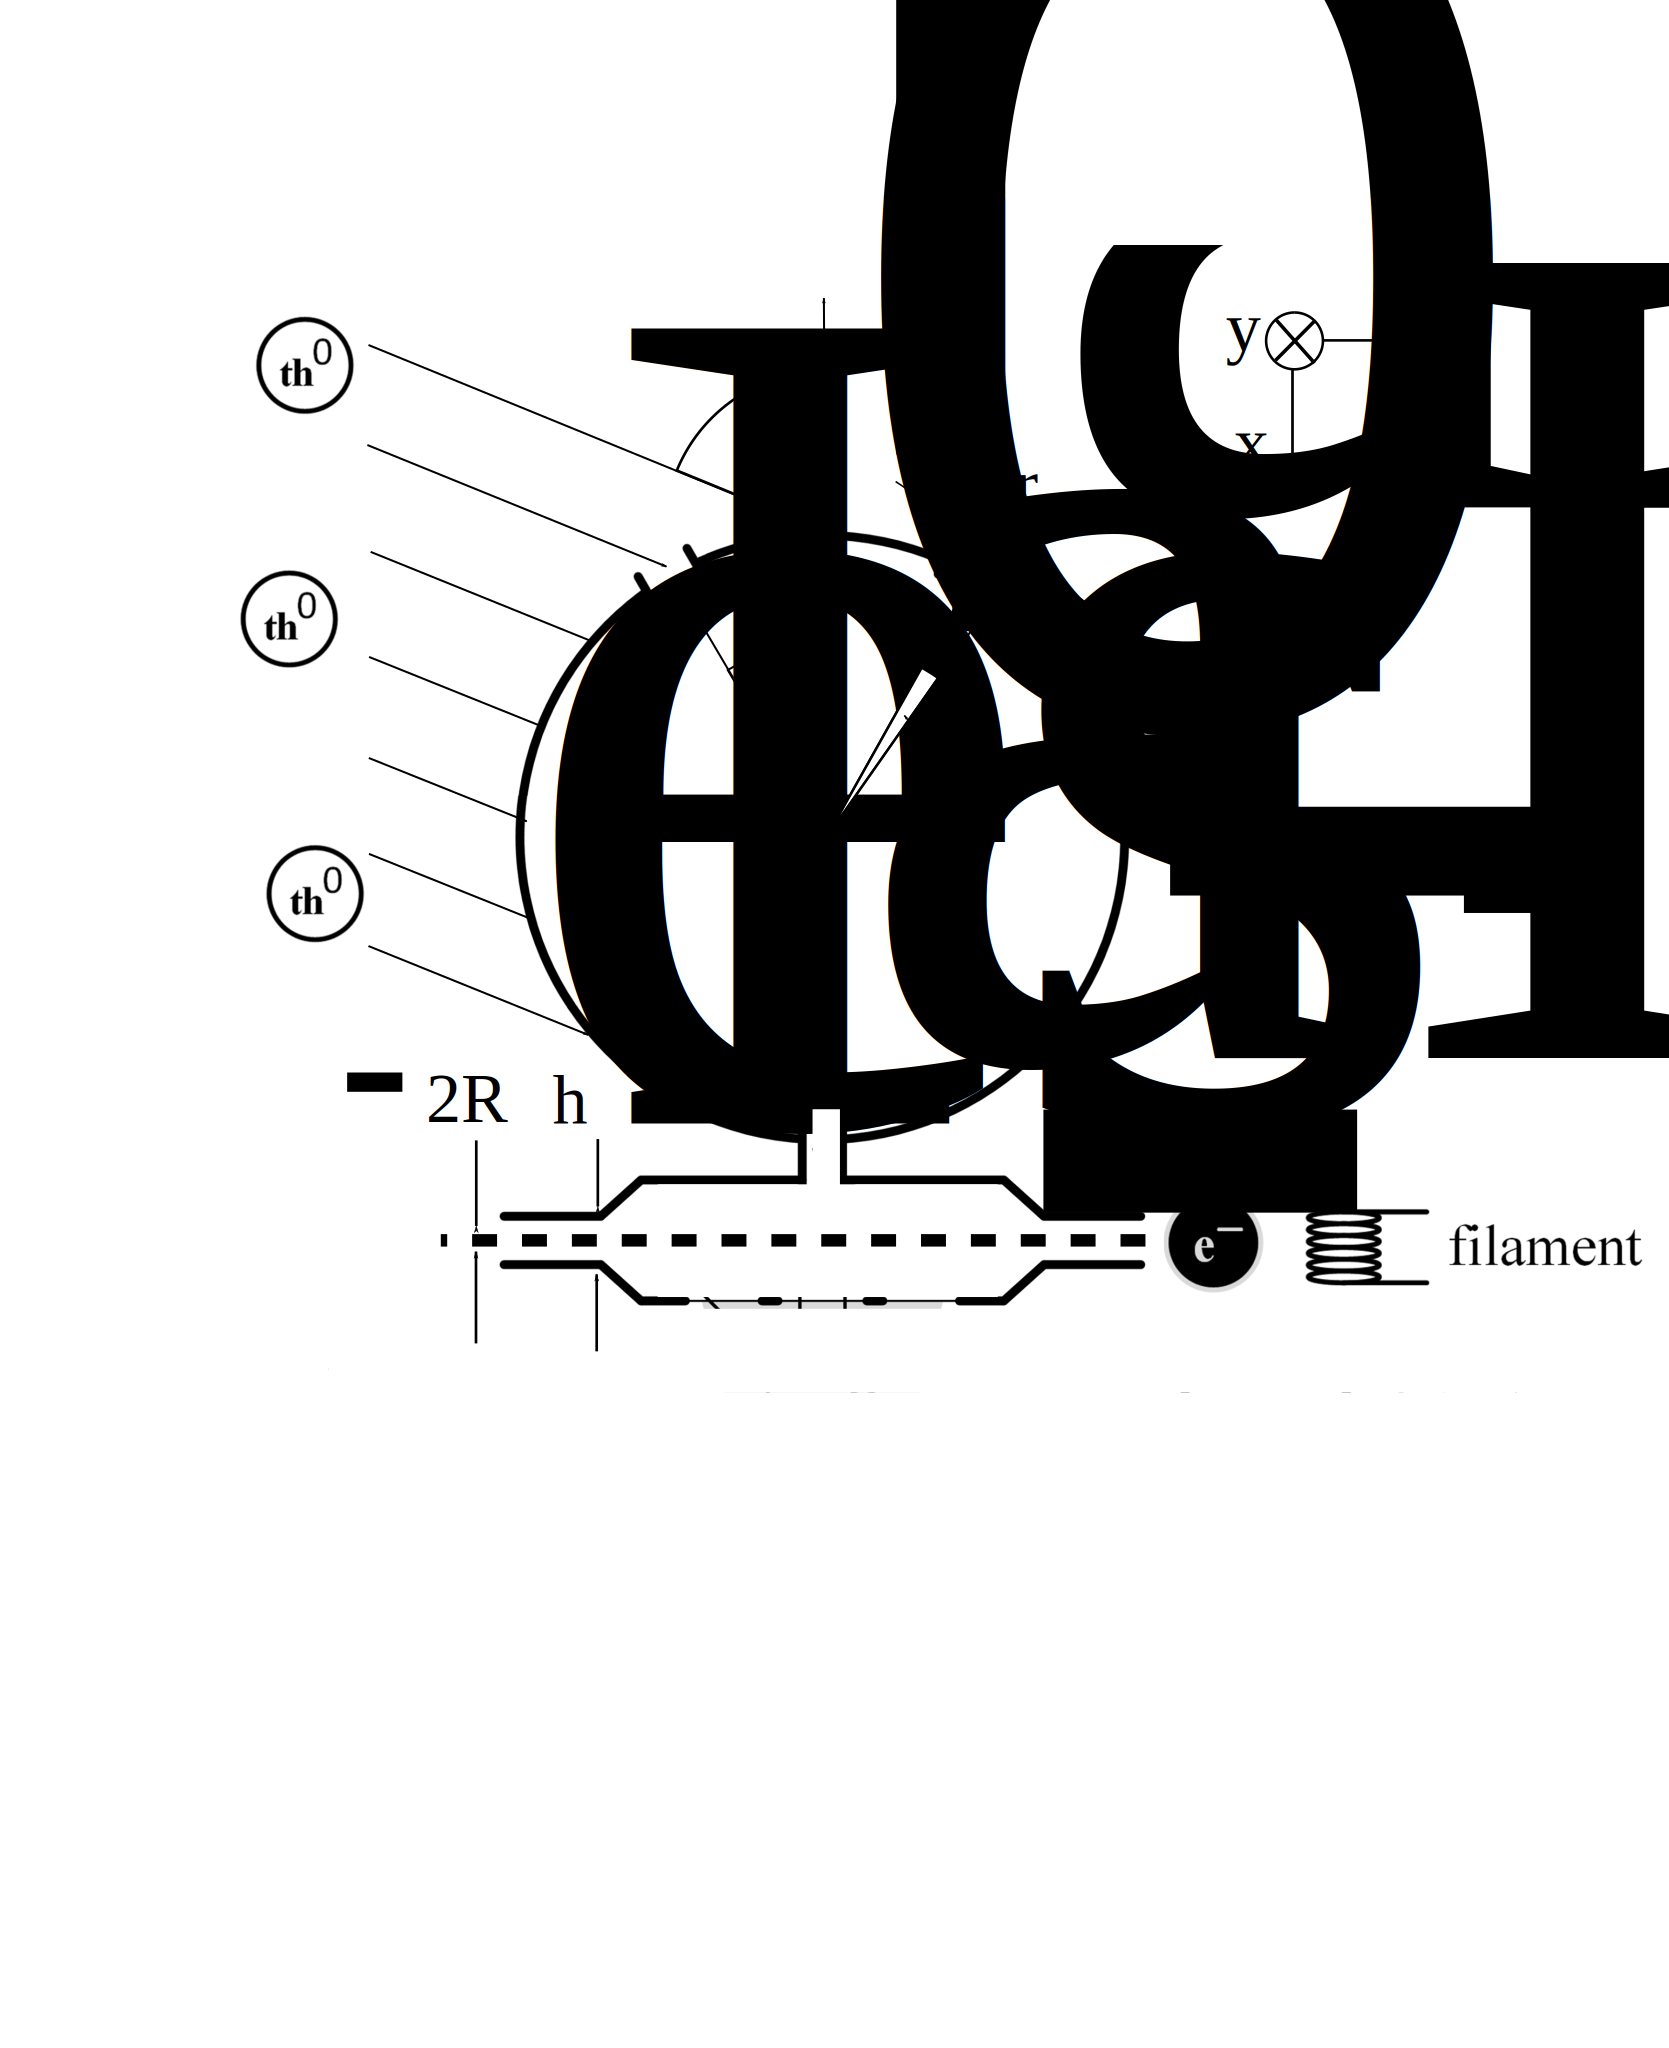
\includegraphics[width= 0.7\textwidth]{Bilder/particleDensEnh.png}
			\caption{Schematics of the antechamber and the ionisation region.}
			\label{fig:thAntIs}
		\end{figure}

%----------------------------------------------------------------------------------------------------
		\subsubsection{Density enhancement Model}\label{subsubsec:Densenhan}
		\begin{table}
			\begin{center}
				\begin{tabular}{|l r |l r |l r|}
					\hline
					$T_a$ 	& 295 K	& $r_{aHi}$	& 2.5\, mm	& $\chi$	& 0\degree \\
					$T_s$ 	& 320 K & $r_{aIs}$ & 2\, mm	& $\theta_0$& 30\degree\\	
					$k$		&	1	& $v_{sc}$	& 2.5\, km/s& $m$		& 18 u\\
					$a$		& 0.23	&			&			&			&	\\
					\hline
				\end{tabular}
			\end{center}
			\caption{Values used for the variation of the different variables of the amplification factor of the antechamber (Eq.\,\eqref{eq:thDensEnhan}).}
			\label{tab:thDensEnhan}
		\end{table}
		
		NIM has an open source entrance where neutral particles and ions enter the ionisation region directly and a closed source entrance where particles enter the ionization region after being thermalized in an antechamber. In this chapter the signal amplification of the closed source entrance is determined. The density enhancement model described in \cite{DensEnhan_Wurz_07} is used and adapted for the geometry of NIM's antechamber. The particle density $n_{cs}$ in the ionization region is:
		\begin{align}
			\frac{n_{cs}}{n_a} &= \sqrt{\frac{T_a}{T_s}}\cdot\frac{k\cdot \sin^2\big(\frac{\omega}{2}\big)\cdot \cos^2\big(\frac{\omega}{2}\big)}{1-k\cdot \cos^2\big(\frac{\omega}{2}\big)}\frac{\big(F(S_1)+ F(S_2)\big)}{2} \frac{r_{aIs}^2\cdot a}{2\cdot r_{aHi}^2 + r_{aIs}^2\cdot a} \label{eq:thDensEnhan}\\
			F(S_i)) &= e^{-S_i^2} + \pi^{1/2}\cdot S_i\cdot\big(1 + {\rm erf}(S_i)\big) \label{eq:F(S)}
		\end{align}
		% cos(chi) = cos(theta_0)cos(theta) +- sin(theta_0)sind(theta)cos(phi)
		With $n_a$ is the particle density of the gas outside the instrument. For the tests in the laboratory $n_a$ is the particle density of then neutral gas beam. In flight it is the particle density of the moons atmosphere. $T_a$ is the temperature of the ambient gas. In the laboratory it is the temperature of the neutral particle beam. $T_s$ is the temperature of the antechamber. $k$ is the probability of a particle being re-emitted after colliding with the antechambers inner surface during thermalization and is close to 1 because otherwise the particle would be absorbed. $\Omega$ is the total solid angle of all openings leading into the antechamber. NIM has two entrance holes with the same hole diameter and therefore the total solid angle $\Omega$ is the sum of the two solid angles of the entrance holes $\Omega'$:
		\begin{equation}
			\Omega = 2\cdot\Omega'
		\end{equation}
		All openings into the antechamber have a circular shape therefore, the solid angle $\Omega$ is replaced by an angle $\omega$ in the x-z-plane to simplify the equation \cite{Hedin_1964}: 
		\begin{align}
			2\pi(1- \cos(\omega)) &= 2\cdot 2\pi(1- \cos(\omega'))\\
			\cos(\omega) &= 2\cos(\omega') -1\\
			\omega &= \cos^{-1}(2\cos(\omega') -1)
		\end{align}
		$\omega'$ is the half angle of one entrance hole (Fig.\,\ref{fig:thAntIs}). $S_i$ in Eq.\,\eqref{eq:F(S)} is the speed ratio along the normal axis of the entrance holes:
		\begin{equation}
			S_i = 
			\begin{cases}
				0, & \cos(\chi \pm \theta_0) < 0\\
				v_{sc}\cdot \cos(\chi + \theta_0)\cdot \sqrt{\frac{m}{2k_B T_a}}, & i=1\\
				v_{sc}\cdot \cos(\chi - \theta_0)\cdot \sqrt{\frac{m}{2k_B T_a}}, & i=2
			\end{cases}
		\end{equation}
		with $v_{sc}$ the velocity of the neutral gas beam relative to the antechamber corresponding to the spacecraft velocity, $m$ the average particle mass of the gas and $k_B$ the Boltzmann constant. $\chi$ is the angle of the test gas relative to the x-axis of the instrument and $\theta_0$ is the angle between the x-axis and the axis normal of the entrance hole. $\chi \pm \theta_0$ is the angle between the normal axis of the entrance hole and the gas influx direction. $\chi \pm \theta_0$ has to be between $\pm 90\degree$ to enter the antechamber which implies that $\cos(\chi \pm \theta_0)$ cannot have negative values. $i=1$ is the index of one of the two entrance hole and $i=2$ is the index of the other entrance hole. The antechamber has three openings for the gas to flow out of the antechamber. The last term in Eq.\,\eqref{eq:thDensEnhan} gives the ratio of how many particle leave the antechamber through the hole connecting the antechamber with the ionization region compared to the amount of particles leaving the antechamber through the two entrance holes. The radius of the entrance holes is $r_{aHi}$ and the radius of the hole connecting the antechamber with the ionization region is $r_{aIs}$. This term takes the molecular flow conductance of the different holes into account. The molecular flow conductance of a thermalized gas is:
		\begin{equation}
			C_0 = A\bar{v}/4
			\label{eq:theoMolFlowCondC0}
		\end{equation}
		with $A$ the cross-section of the opening and $\bar{v}$ the average velocity of the thermalized gas flowing through that opening. This formula is only valid in case the length of the tube is close to zero. Otherwise, the transmission probability $a$ has to be added resulting in:
		\begin{equation}
			C = C_0 \cdot a
			\label{eq:theoMolFlowCondCEff}
		\end{equation}
		The transmission probability depends on the length-to-radius ratio $L/R$ of the opening. D. van Essen and W. Chr. Heerens compared different approaches to determine the transmission probability and give values for specific length-to-radius ratios \cite{molFlowTubeTransm_Essen1976}. The approximation which comes closest to reality is the one by Nawyn and Meyer. To calculate the transmission probability for any length-to-radius ratio, this data was fitted with the following function:
		\begin{equation}
			a = y_0 + A_1\left(1-e^{-\frac{L/R}{t_1}}\right) + A_2\left(1-e^{-\frac{L/R}{t_2}}\right)
			\label{eq:MolFloConFitFunc}
		\end{equation}
		The fit parameters are listed in Table\,\ref{tab:thMolFloConFiPara}.
		\begin{table}[h!]
			\begin{center}
				\begin{tabular}{l r| l r }
					$A_1$	& $-0.48 \pm 0.01$ & $t_1$	& $7.4 \pm 0.3$	\\
					$A_2$	& $-0.45 \pm 0.01$ & $t_2$	& $1.13 \pm 0.04$ \\
					$y_0$ 	& $0.998 \pm 0.001$	& &\\
				\end{tabular}
			\end{center}
			\caption{Fit parameters of Eq.\,\eqref{eq:MolFloConFitFunc}.}
			\label{tab:thMolFloConFiPara}
		\end{table}	
		For the two gas entrance openings of the antechamber $a$ is 1 because they have a sharp edge and therefore the length of the opening is close to zero. The opening between the antechamber and the entrance has a length-to-diameter ratio of 8 resulting in a $a$ of 0.23. The amount of gas flowing through this opening relative to the total outflow is:
		\begin{align}
			G_{open} & = \frac{C_{aIs}}{C_{aIs} + 2\cdot C_{aHi}} \label{eq:GAntOpen}\\
			G_{open} & = \frac{\frac{r_{aIs}^2\cdot a\cdot \bar{v}}{4}}{\frac{r_{aIs}^2\cdot a\cdot \bar{v}}{4} + 2\frac{r_{aHi}^2\cdot \bar{v}}{4}}\\
			G_{open} &= \frac{r_{aIs}^2\cdot a}{r_{aIs}^2\cdot a + 2\cdot r_{aHi}^2}
		\end{align}
		With $r_{aIs} = 2\,\si{\milli\meter}$ and $r_{aHi} = 2.5\,\si{\milli\meter}$ resulting in $G_{open} = 0.067$ meaning that about 6.7\% of all particles entering the antechamber actually reach the ionization region due to losses of the geometry.\\
		
		In the following section the different parameters of the density enhancement equation Eq.\,\eqref{eq:thDensEnhan} were varied to determine their impact. For this analysis the particle density in the ionization region $n_{cs}$ was divided by the particle density of the test gas $n_a$ outside of the antechamber and $n_a$ was set 1 to get the amplification of the antechamber. For this analysis the parameters were set according to Table\,\ref{tab:thDensEnhan} unless otherwise mentioned. The temperatures are the ones used in the laboratory. The used particle velocity was 2.5\,\si{\kilo\meter\per\sec} because it is velocity of the spacecraft in Ganymede orbit and the velocity at which most of the measurements will be done.\\		
		The first parameter which was varied was the gas temperature $T_a$. This temperature can be varied between 0 and 1000\,\si{\kelvin} without significantly influencing the gain of the antechamber (Fig.\,\ref{th:densEnhTaTs}). When looking closer, a slight increase in gain is observed with increasing temperature.\\
		The temperature of the antechamber $T_s$ has a bigger impact on the gain. Ideally this temperature should be as low as possible to slow down the particles when they hit the chamber walls. When the temperature of the antechamber is too low, the gas condenses at the antechamber walls. Therefore the antechamber is kept at temperatures higher than -17\,\si{\degreeCelsius} during measurements. \notes{Continue here!!!}\\
		\begin{figure}[h!] % T_a T_s
			\centering
			\includegraphics[width= .7\textwidth]{Bilder/Ta_Ts.png}
			\caption{Gain $n_{cs}/n_a$ as a function of the antechamber the ambient gas temperature $T_a$ and the temperature of the antechamber wall $T_s$ according to Eq.\eqref{eq:thDensEnhan}.}
			\label{th:densEnhTaTs}
		\end{figure}
		The next parameter is the radius $r_{aIs}$ of the hole connecting the antechamber with the ionisation region. When the hole gets bigger, also the amount of gas flowing into the ionisation region increases as it can be seen in Fig.\,\ref{th:densEnhraHiraIs}. The radius of the entrance holes $r_{aHi}$ should be small to reach a high gain. This has two reasons: When the entrance holes are big compared to the hole connecting the antechamber with the ionisation region, a big amount of gas flows out through the entrance holes. The size of the entrance holes has also an impact on the opening angle $\omega$. In the first designs of such antechambers, the ionisation and counting of the particles happened in the antechamber itself \cite{Hedin_1964}. Therefore the antechamber needed only one opening. Our instrument has two entrances for particles. One to measure them directly without any interaction with the instrument surface (open-source channel) and a closed-source entrance through the antechamber to amplify the signal. Due to the flyby trajectories of the space craft the antechamber has to entrance holes with angle $\theta_0 = 30\degree$ relative to the x-axis of the instrument.\notes{Rewrite}
		When having only one big entrance hole, the gas gets easily reflected and leaves the antechamber before being counted in the antechamber. Therefore a small opening is favoured over a big opening. From that perspective, the biggest gain is achieved when the radius of the entrance hole is 0 ergo the entrance hole is closed. That's the limitation of Eq.\,\eqref{eq:thDensEnhan} is. It does not take into account that at a certain radius of the opening, the gain should decrease because not enough particles enter the chamber to get amplified.\\
		\begin{figure}[h!] % raHi raIs
			\centering
			\includegraphics[width= .7\textwidth]{Bilder/raHi_raIs.png}
			\caption{Gain $n_{cs}/n_a$ of the antechamber as a function of the entrance hole radius $r_{aHi}$ and the radius connecting the antechamber with the ionisation region $r_{aIs}$.}
			\label{th:densEnhraHiraIs}
		\end{figure}
		It is very important to take materials with a high particle reflection coefficient $k$ for the coating of the antechamber' s inner surface. The particle reflection coefficient gives the probability of a particle being re-emitted when hitting the surface thus this value has to be close to 1. For our antechamber we used gold because it is electrically conductive preventing the surface from charging in the strong radiation field of Jupiter and it is chemically inert and thus there is a low probability of building chemical bonds with the test gas. Fig.\,\ref{th:densEnhk} shows the amplification of the antechamber in dependence of $k$. When changing $k$ by 1\textperthousand\, this already has a huge impact on the amplification. The impact of $k$ also depends on $\omega$. A small $\omega$ implies a big surface area with which the particles can interact before leaving the antechamber. The more interactions with the antechamber surface are possible, the bigger is the influence of $k$. For our antechamber $\omega$ is about 5.06\,\si{\degree} which is very small and therefore a small change in $k$ has a big impact on the gain.\\
		\begin{figure}[h!] % k
			\centering
			\includegraphics[width= .7\textwidth]{Bilder/k.png}
			\caption{Gain $n_{cs}/n_a$ of the antechamber as a function of the particle reflection coefficient $k$.}
			\label{th:densEnhk}
		\end{figure}
		Fig\ref{th:densEnhm} shows the amplification of the antechamber in dependence of the particles unit mass\,[u]. The figure shows that particles with higher unit mass get amplified more and are therefore easier to detect.\\
		\begin{figure}[h!] % mass
			\centering
			\includegraphics[width= .7\textwidth]{Bilder/m.png}
			\caption{Gain $n_{cs}/n_a$ of the antechamber as a function of the particle mass $m$.}
			\label{th:densEnhm}
		\end{figure}
		Fig.\,\ref{th:densEnhvelo} shows the amplification of the antechamber in dependence of the spacecraft velocity for different species. We expect H\textsubscript{2}O and different radiolysis radiolysis products such as H\textsubscript{2}, O\textsubscript{2} or HO. Absorption lines in the near infrared recorded by the Near Infrared Mapping Spectrometer (NIMS) on board of the Galileo spacecraft indicate CO\textsubscript{2} bond to other solid materials in the soil. Sulphur is part of the plasma. The sulphur compounds are therefore a result of the ion bombardment on the moons surface. Sulphur reacts with water resulting in various different compounds such as sulphur dioxide (SO\textsubscript{2}) or sulphuric acid (H\textsubscript{2}SO\textsubscript{4}) \cite{Collins_2014}. \notes{include Audrey's paper if it gets finished in time.}
		Fig.\,\ref{th:densEnhvelo} shows that with increasing flyby velocity, the particles get more amplified. Species with higher masses are stronger amplified than light particles as it was already shown also in Fig.\,\ref{th:densEnhm}.\\
		\begin{figure}[h!] % velocity
			\centering
			\includegraphics[width= .7\textwidth]{Bilder/velocity.png}
			\caption{Gain $n_{cs}/n_a$ of the antechamber as a function of the spacecraft velocity $v_{sc}$ for different species expected in the moons atmospheres.}
			\label{th:densEnhvelo}
		\end{figure}
		Fig.\,\ref{th:densEnhChiTheta} shows the amplification in dependence of different particle influx angles $\chi$. $\chi$ is measured in the x-/y- plane (Fig.\,\ref{fig:thAntIs}). The function was evaluated for different positions of the entrance holes. The minimal angle the two entrance hole can be apart from each other without overlapping is 3.6\si{\degree}. The holes of the PFM are at $\theta_0 = \pm30\,\si{\degree}$. With that configuration the biggest signal intensity is measured with a spacecraft ramp direction of 0\si{\degree}. When the two holes are at $\pm$60\si{\degree} it results in a plateau between $\pm$60\,\si{\degree} and also a wider angular range at which NIM is sensitive. This is an interesting feature under certain circumstance. For our purpose it is unnecessary because the spacecraft blocs the field of view (FoV) for angles bigger than 100\degree (see also Chap.\,\ref{subsubsec:Calfly}).
		\begin{figure}[h!] % chi theat
			\centering
			\includegraphics[width= .8\textwidth]{Bilder/Chi_theta0.png}
			\caption{Gain $n_{cs}/n_a$ of the antechamber as a function of the gas influx direction $\chi$ for different positions of the two entrance holes $\theta_0$. $\theta_0=30\degree$ is the position of the holes in flight configuration.}
			\label{th:densEnhChiTheta}
		\end{figure}
		
%-------------------------------------------------------------------------------------------		
		\subsubsection{Callisto Flyby}\label{subsubsec:Calfly}
	
		\begin{figure}[h!]
			\centering
			\includegraphics[width=.8\textwidth]{Bilder/Callisto_flyby_schematic.png}
			\caption{Schematics of one of the flybys at Jupiter's moon Callisto.}
			\label{fig:CalflybySchem}
		\end{figure}
				
		\begin{figure}[h!]
			\centering
			\includegraphics[width = .7\textwidth]{Bilder/NIM_pointing_2031JAN15185200.png}
			\caption{Fourth Callisto flyby of trajectory 141a \cite{SOC_Crema3p2} 1\,h before closest approach 15'600\,km away from Callisto.}
			\label{fig:FlybyCal1852}
		\end{figure}
		\begin{figure}[h!]
			\centering
			\includegraphics[width = .7\textwidth]{Bilder/NIM_pointing_2031JAN15194200.png}
			\caption{Fourth Callisto flyby of trajectory 141a \cite{SOC_Crema3p2} 10\,min before closest approach 1'560\,km away from Callisto.}
			\label{fig:FlybyCal1942}
		\end{figure}
		\begin{figure}[h!]
			\centering
			\includegraphics[width = .7\textwidth]{Bilder/NIM_pointing_2031JAN15194700.png}
			\caption{Fourth Callisto flyby of trajectory 141a \cite{SOC_Crema3p2} 5\,min before closest approach 580\,km away from Callisto.}
			\label{fig:FlybyCal1947}
		\end{figure}
		\begin{figure}[h!]
			\centering
			\includegraphics[width = .7\textwidth]{Bilder/NIM_pointing_2031JAN15195200_tilt.png}
			\caption{Fourth Callisto flyby of trajectory 141a \cite{SOC_Crema3p2} closest approach 200\,km away from Callisto with the solar panels oriented toward the sun to maximizes power generation of the spacecraft.}
			\label{fig:FlybyCal1952sol}
		\end{figure}
		\begin{figure}[h!]
			\centering
			\includegraphics[width = .7\textwidth]{Bilder/NIM_pointing_2031JAN15195200.png}
			\caption{Fourth Callisto flyby of trajectory 141a \cite{SOC_Crema3p2} closest approach 200\,km away from Callisto.}
			\label{fig:FlybyCal1952}
		\end{figure}
		\begin{figure}[h!]
			\centering
			\includegraphics[width = .7\textwidth]{Bilder/NIM_pointing_2031JAN15195700.png}
			\caption{Fourth Callisto flyby of trajectory 141a \cite{SOC_Crema3p2} 5\,min after closest approach 640\,km away from Callisto.}
			\label{fig:FlybyCal1957}
		\end{figure}
		Fig.\,\ref{fig:FlybyCal1852}\,- Fig.\,\ref{fig:FlybyCal1957} show the changing FoV of the NIM instrument at different times during the fourth Callisto flyby of trajectory 141a \cite{SOC_Crema3p2}. The reference coordinate system for these graphics is the ecliptic coordinate system. During the flyby, the spacecraft changes its orientation in reference to that coordinate system leading to a distortion of the different objects in the figures. The entrance holes of the antechamber are blue circles, the FoVs of the entrance holes are marked as dashed blue lines, the entrance slit is the blue band with the sinusoidal shape. The solar panels and the antenna which bloc part of the FoV of NIM are marked in red. The gas inflow direction is marked as an orang star. Fig.\,\ref{fig:FlybyCal1852} shows the FoV 1\,h before closest approach 15'600\,km above Callisto's surface. The gas inflow direction is in between the two entrance holes. The black doted line on the moons surface marks the day/night separation line. As the spacecraft moves closer to the moon, the gas inflow direction moves towards the entrance slit. 5\,min before closest approach, NIM changes from thermal to neutral mode (Fig.\,\ref{fig:FlybyCal1947}) to be ready for the neutral mode measurements. At this time, the gas inflow direction is still in the FoV of the antechamber. The time window for measuring with the neutral gas mode is very narrow. Already 5\,min after closest approach, the gas inflow direction is below the FoV of the neutral gas channel (Fig.\,\ref{fig:FlybyCal1957}). Therefore, the time to switch from thermal to neutral mode has to be very short to minimize the number of lost measurements. These measurements are very crucial because the closer the spacecraft gets to the moon's surface, the higher is the exospheric pressure and therefore the signal intensity.\\
		The spacecraft structure blocs angles higher than 100\si{\degree}. The gas striking the spacecraft sputters particles from the spacecraft's surface. NIM is not able to determine if these particles are part of the moons exosphere of if they originate from the spacecraft. When the gas inflow direction reaches angles higher than 100\si{\degree} NIM starts measuring background. The solar panels are adjusted perpendicular to the sun to maximize power generation. 10\,min before closest approach, the solar panels are tilted to leave open the FoV of NIM to measure with the neutral gas mode. In case the solar panels would stay perpendicular to the sun, the gas would graze the surface of the solar panel as it is shown in Fig.\,\ref{fig:FlybyCal1952sol}. Fig.\,\ref{fig:FlybyCal1952} shows the same scenario but with the solar panels tilted to leave open NIM's FoV of the neutral gas channel.\\
		Fig.\,\ref{fig:densEnhChiFlyby} shows the gain of the antechamber with the total FoV of the two entrance holes marked as red area $\pm$30\degree around the position of the two entrance holes. The orange stars mark the gas inflow direction for the various scenarios mentioned before.
		\begin{figure}[h!]
			\centering
			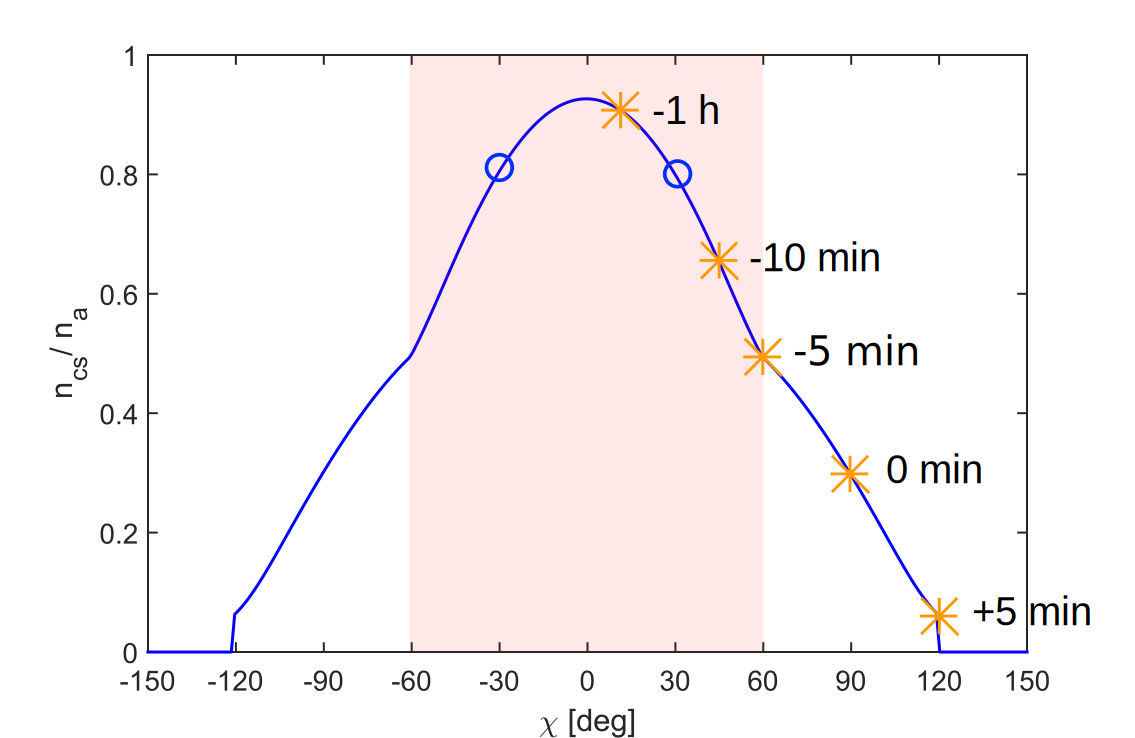
\includegraphics[width=.8\textwidth]{Bilder/Chi_theta0_flyby.png}
			\caption{Gain $n_{cs}/n_a$ of the antechamber in dependence of the gas influx direction $\chi$. The blue circles mark the entrance hole positions and the red area marks the FoV of the entrance holes. The stars mark the gas influx direction from 1\,h before until 5\,min after closest approach of trajectory 141a \cite{SOC_Crema3p2}.}
			\label{fig:densEnhChiFlyby}
		\end{figure}
		The main gas inflow direction varies for the different flybys. One time the gas comes from positive and one time from negative $\chi$ direction. Therefore, it was decided to make two entrance holes to allow measurements with angles different to the main direction to enlarge the FoV of the antechamber. The holes should also not be too close at the entrance because structures of the spacecraft bloc angles bigger than 100\degree and an amplification of such big angles would be useless.
		
		
%----------------------------------------------------------------------------------		
		\subsubsection{Shutter Performance} \label{subsubsec:motorflow}
		NIM has a shutter to close the entrance to the antechamber. This shutter is mounted between the ion source and the antechamber (Fig.\,\ref{fig:shutterMotor} left). When the shutter is open, the gas flows right through the hole into the ion source. When the shutter is closed, the hole moves to the side as it is indicated in Fig.\,\ref{fig:shutterMotor} right. Because the shutter does not close the gag perfectly, still a small amount of gas flows around the shutter into the ionisation region. In the following section, the geometry factor $G_{close}$ of the antechamber is determine when the shutter is closed.\\
		\begin{figure}[h!]
			\begin{subfigure}{0.5\textwidth}
				\centering
				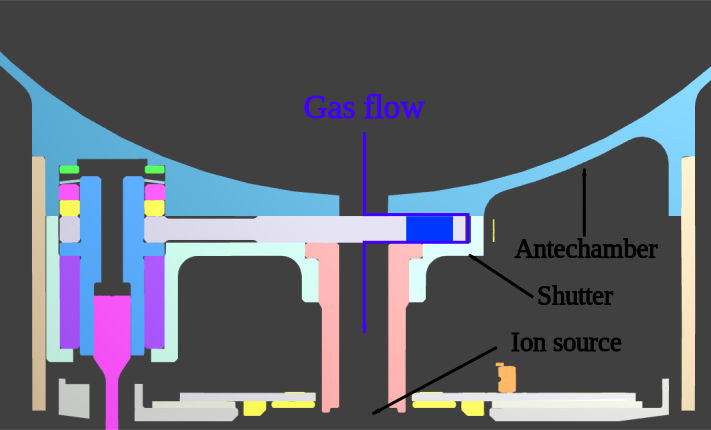
\includegraphics[width=\textwidth]{Bilder/Shutter_sideview.png}
			\end{subfigure}
			\begin{subfigure}{0.5\textwidth}
				\centering
				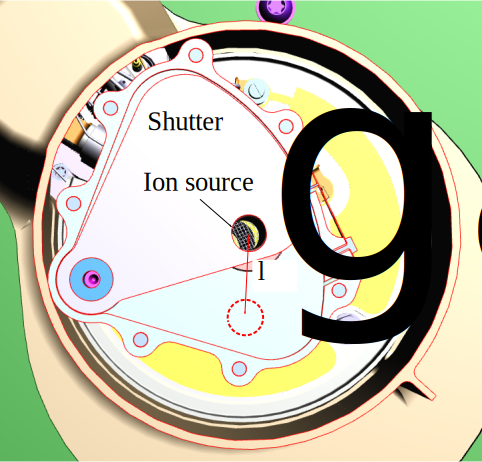
\includegraphics[width=.8\textwidth]{Bilder/Shutter_topview.png}
			\end{subfigure}
		\caption{Shutter Motor. Left: side view with shutter closed. Right: Top view with open shutter. When the shutter is closing the central hole moves to the red position.}
		\label{fig:shutterMotor}
		\end{figure}
		The molecular flow conductance is:
		\begin{equation}
			C = \frac{A\cdot\bar{v}\cdot a}{4}
		\end{equation}
		With $A$ the cross-section of the tube, $\bar{v}$ the average velocity of the thermalized gas flowing through the opening and $a$ the transmission probability depending on the length-to-diameter ratio of the tube. When the shutter is closed, the conductance of the tube $C_{tot}$ is divided into four terms: The conductance of the upper part of the tube $C_{top}$, the conductance of the gap between the shutter and pocket $C_{gap}$, the conductance of the hole in the shutter $C_{hole}$ and the conductance of the lower part of the tube connecting the antechamber with the ionization region $C_{bot}$ (Fig.\ref{fig:shutterMotor} left):
		\begin{align}
			C_{top}  &= \frac{r_{aIs}^2\cdot\pi\cdot\bar{v}\cdot a_{top}}{4}\\
			C_{gap}  &= \frac{2\cdot r_{aIs}\cdot \pi \cdot h_{gap}\cdot\bar{v}\cdot a_{gap}}{4}\\
			C_{hole} &= \frac{r_{aIs}^2\cdot\pi\cdot\bar{v}\cdot a_{hole}}{4}\\
			C_{bot}  &= \frac{r_{aIs}^2\cdot\pi\cdot\bar{v}\cdot a_{bot}}{4}
		\end{align}
		\begin{table}[h!]
			\begin{center}
				\begin{tabular}{l r| l r }
					$a_{top}$	& 0.73 	& $h_{top}$		& 1.5\,mm	\\
					$a_{gap}$	& 0.07 	& $h_{gap}$		& 0.01\,mm \\
					$a_{hole}$ 	& 0.67 	& $h_{hole}$ 	& 2\,mm\\
					$a_{bot}$ 	& 0.28 	& $h_{bot}$ 	& 12\,mm\\
					$r_{aIs}$ 	& 2\,mm & $l_{gap}$ 	& 7\,mm\\
				\end{tabular}
			\end{center}
			\caption{Nominal transmission probabilities $a_i$, tube heights $h_i$, tube radius $r_{aIs}$ and minimal gap length $l_{gap}$ when the shutter between the antechamber and the ion-source is closed.}
			\label{tab:thMolFloConMotClosPara}
		\end{table}	
		With $a_{i}$ the transmission probabilities of the different sections (Eq.\,\eqref{eq:MolFloConFitFunc}), $h_i$ the height of the different sections, $r_{aIs}$ the radius of the antechamber hole and $l_{gap}$ the minimal distance between the hole in the shutter and the tube connecting the antechamber with the ion-source. The nominal values for these parameters are listed in Table\,\ref{tab:thMolFloConMotClosPara}. The average velocity $\bar{v}$ will cancel out later in the derivation of the geometry factor. The conductance of the tube $C_{tot}$ is:
		\begin{equation}
			\frac{1}{C_{tot}} = \frac{1}{C_{top}} + \frac{2}{C_{gap}} + \frac{1}{C_{hole}} + \frac{1}{C_{bot}}
		\end{equation}
		The conductance of one of the entrance holes of the antechamber is:
		\begin{equation}
			C_{aHi} = \frac{r_{aHi}^2\cdot\pi\cdot\bar{v}}{4}
		\end{equation}
		The geometry factor of the tube when the shutter is closed $G_{close}$ is:
		\begin{equation}
			G_{close} = \frac{C_{tot}}{C_{tot} + 2\cdot C_{aHi}}
		\end{equation}
		\begin{figure}[h]
			\centering
			\includegraphics[width=.8\textwidth]{Bilder/ShutGapSizeSigDamp.png}
			\caption{Damping factor $G_{open}/G_{close}$ of the shutter as a function of the gap size $h_{gap}$ of the gap between the shutter and antechamber.}
			\label{fig:ShutGapSizeSigDamp}
		\end{figure}
		The gap between the shutter and the antechamber has to be very thin to seal the hole when the shutter is closed. Fig.\,\ref{fig:ShutGapSizeSigDamp} shows the damping factor $G_{open}/G_{close}$ as a function of the gap size $h_{gap}$. With increasing gap size, the damping factor reduces significantly. The requirement was to damp the signal by a factor 1000 when the shutter is closed. With the nominal gap size of 0.01\,mm, the shutter damps the signal by a factor 600. When the gap size is about 0.1\,mm the damping factor is only about 25. This may can happen when the shutter is not properly fabricated and the tolerances are therefore bigger than originally designed.\\
		When measuring with the open source channel, a small amount of gas will enter the ion-source through the antechamber. The open source slit is in the y-/z-plane and therefore $\chi$ is 90\si{\degree} (Fig.\ref{fig:thAntIs}). When the shutter is closed, about 0.05\% of the signal originates from the antechamber.
		
		%In this approximation the assumption was that the gas will take the shortest distance between the antechamber and the ion-source. In reality it will flow around the shutter and the signal will be damped even more because with increasing distance the gas has to flow, it get damped more.
		

		\subsubsection{Pressure calibration of the NIM Sensor}
		% This chapter comes after the calculation of the detector gain because the gain of the detector is part of the pressure calculation. Proper error estimation of the paramaeters as far as possible.
		% More detailed explanation about the NIM ion source, function of the different specific electrodes. Or explain it later in detail when discussing the simulations in detail. See paper as a guide line. Especially for the ion storage part.
		
		
		
		\textcolor{red}{see also density enhancement book for that derivation!!!}
		To calculate the number of ions produced in the ion source we use:
		\begin{equation}
		I_{ion} = \beta\cdot Q_{ion}\cdot L\cdot n\cdot I_{em}
		\end{equation}
		With $\beta$ the extraction efficiency which is 1, % Noch schauen auf welchen Wert wir diese setzen wollen. 1= sehr gute Quelle, 0.01 = 1mus/100mus = Pulslänge Pulser/ Länge 1 Zyklus. Noch diskutieren, welche Werte beta haben kann oder einfach etwas setzen? Da die ersten Messresultate gut sind, würde ich eher auf 1 setzen. Abschätzung? Auf Unterschiede beim Spannungsset hinweisen -> beeinflusst beta massgeblich.
		$L$ as the effective ionising path in our case 4~\si{\milli\metre}, $n$ the particle density, $I_{em}$ the electron emission current from the filament and $Q_{ion}$ the ionising cross section. The cross sections of species used in our calibration can be found in table % Ref. auf Tabelle und nur auf Stefans Diss verweisen oder die 4 Originalpaper zusammen suchen. Tabelle einfügen.
		
		\textcolor{red}{Write something about the radiation shielding concept? Or just make a reference to the paper because it gives an overview over the concept as far as it is necessary.}
		
		\subsubsection{Detector Parameters} % Clean up this chapter when finalizing the detector chapter. Finalize the theory part and the explanation of the workmanship of the detector housing.
		% All relevant parameters
		% Gain
		% dead time, R, C, number of channels. Calculation of the number of channels out of the data sheet (Diss Maike) charging behaviour. Is this really needed for the analysis I do? I case I should have to test with the FS, it would be nice to include that calculation and the timing resulting out from that. Otherwise it is just a nice part of theory but is not used for anything. Set up something, just that the chapter is completed (sort of).
		% Compare the performance of the diode with the performance of the resistor. Depending on the results, find arguments.. No time for that :(
		
		In this section we calculated some important parameters of the detector such as the dead time and the gain. % And further values if needed.
		
		\textbf{Dead time}\\
		
		\begin{figure}[h]
			\centering
			\includegraphics[width=.4\textwidth]{Bilder/MCP_hex.jpg}
			\caption{MCP honeycomb structure \cite{Diss_Neuland}.}
			\label{fig:MCPhex} % Ref. Maike Diss
		\end{figure}
		The number of channels $N$ of an MCP is its active area $A_{act}$ divided by the area of one channel $A_{hex}$. The MCP has a honeycomb like structure (Fig.\,\ref{fig:MCPhex}). Thus, the area of one channel is the area of a hexagon:
		\begin{equation}
			N = \frac{A_{act}}{A_{hex}} = \frac{2\cdot\pi r^2_{act}}{\sqrt{3}p^2}
		\end{equation}
		$r_{act}$ is the radius of the active area of the MCP which is for our MCPs 8\,\si{\milli\meter} and p is the distance between the centres of two channels which is 6\,\si{\micro\meter}. This results in $1.6\cdot10^6$ channels.\\
		The resistance of a single channel is the resistance of the whole MCP plate $R_{MCP}$ times the number of channels $N$:
		\begin{equation}
			R_{ch} = R_{MCP}\cdot N
		\end{equation}
		Its resistance depends on the voltage applied over the plate. For a nominal voltage of 1000\,\si{\volt} $R_{MCP}$ is $\sim$70\,\si{\mega\ohm} resulting in channel resistance of about $10^{14}$\,\si{\ohm}.\\
		The MCPs consist of two different materials: the structure (grey) consists of a type of lead glass and the hole, which can be approximated with vacuum (white) (Fig.\ref{fig:MCPhex}). The area of the structure is equal to the area of the hexagon $A^{hex}_{ch}$ minus the area of the channel hole $A^{hole}_{ch}$. the capacitance of one channel $C_{ch}$ is:
		\begin{equation}
			C_{ch} = \frac{\epsilon_0  (\epsilon_r \cdot (A^{hex}_{ch} - A^{hole}_{ch})+ A^{hole}_{ch})}{l_{ch}}
		\end{equation}
		With $\epsilon_0$ the vacuum permittivity, $\epsilon_r$ the relative permittivity of lead glass and $l_{ch}$ the MCP thickness which is 0.3\,\si{\milli\meter}. The relative electric permittivity depends strong on the conditions under which the material is used for example under which voltage, frequency or temperature the MCPs are used. Furthermore, the manufacturer does not give details about the material characteristics as it is a company secret. In \cite{Diss_Neuland} is an analysis of different values for $\epsilon_r$ found in literature. These values are between 6 and 20. With these values, the resulting capacity is 5\,\si{\atto\farad} per channel. The dead time of a single MCP channel is the channel resistance $R_{ch}$ times the channel capacitance $C_{ch}$:
		\begin{equation}
			\tau = R_{ch}\cdot C_{ch}
		\end{equation}
		This results in a dead time of 500\,\si{\micro\second}. A typical waveform has a duration of about 100\,\si{\micro\second}. When an ion hits a channel, this channel would be blind for the next five waveforms. With $1.6\cdot10^6$ channels and assuming a uniform distribution of particles on the MCP surface, saturation is assumed at particle rates higher than $10^9$ particles/\si{\second}. % Do we really want to have this in? Because saturation really starts at 10^6 #/sec already due to other effects. If so, make at least a short remark to which effects.
		\begin{equation}
			U(t) = U_0\cdot(1- e^{-t/\tau})
		\end{equation}
		It is the time needed to recharge a single channel to approximately 63\% of its original charge. After $5\tau$ 99\% of the original charge is replenished. % Is only half true. Only under the assumption that all of the charge is extracted out of the MCP. May later further discussion and revision.
		
		
		
		% Atempt to calculate the acctual voltage drop of the MCP voltage in dependence of the count rate by taking into account the capacitorloading curve and the option of a possible paralyzability of the detector. To make that properly, a simulation would be necessary. Not relevant.
		
		\begin{comment}
			1 particle with tau as the dead time. Voltage of 1 channel when 1 particle hits the channel. We assume, that we do not get into saturation. At what particle rate does the voltage start to break down. When a particle hits the channel when the voltage is not full replenished, it empties the channel again.
			For a first approximation, wait for 5*tau until 99% of the voltage is recovered.
			Uch(tion) = U_0\cdot(1- e^{-tion/\tau}) % tion is the time when an ion triggers a signal.
			Assumption of this formula is that one ion empties the hole channel -> it extracts alls the current in the channel -> all ions should have the same amount of current = the same gain.
			
			1.6*10^6 particles/second -> 1#/6*10^-7 sec.
			
			ion arriving rate is constant and the ions distributed homogenious over the MCP plate
					
			tZero = countRate % time which resets your voltage to 0V of the channel.
			t_rate = 5*tau.
			Umcp = sum(Uch)/#Channels
			
			Temporal the count rate is much higher than the value averaged over 1 sec. -> The gain will drop within one spectrum but will recover to a certain amount until the next spectrum. This calculation looks at total paralyzability.
			
			See Simulations by Maike for the whole calculation -> also the gain drop is displayed there. Just summarize it here because it is interesting :) and it also gives sort of an approximation of the voltage drop.
			-> Weekend
			
		\end{comment}

		\textbf{Gain}\\
		% Check all variables, if it is consistent. Finish this chapter properly
		The following derivation is strongly based on the lecture notes of \cite{LecNot_Wurz2017}.	When an incoming particle hits the MCP channel wall there is a certain chance that it ejects an electron out of the channel wall. By applying an electric field $E$ over the MCP plate, this electron gets accelerated until it hits the opposite wall, where it ejects more electrons:
		\begin{equation}
			E = \frac{U_{MCP}}{l} = \frac{F}{q_0} = \frac{a m_e}{q_0}
		\end{equation}
		With $U_{MCP}$ the voltage applied over the MCP, $l$ the channel length, $F$ the force applied on the electron, $q_0$ the elementary charge and $m_e$ the mass of the electron. The acceleration of the electron is:		
		\begin{equation}
			a = \frac{U_{MCP}\cdot q_0}{l\cdot m_e}
		\end{equation}
		The distance $s$ an electron travels along the channel until it reaches the channel wall is:
		\begin{equation}
			s = \frac{1}{2}at^2 = \frac{U_{MCP}\cdot q_0\cdot t^2}{l\cdot m_e\cdot 2}
			\label{eq:DetGainChFlightDist}
		\end{equation}
		With $t$ the flight time of an electron until it hits the wall again. Assuming the initial velocity $v_{init}$ of the initial secondary electron is perpendicular to the channel wall, the flight distance until it hits the opposite channel wall is the channel diameter $d$. $t$ can be written as:
		\begin{equation}
			t = \frac{d}{v_{init}}
			\label{eq:DetGainChFlightTime}
		\end{equation}
		$v_{init}$ can be derived out of the electron's initial kinetic energy $U_{init}$:
		\begin{equation}
			U_{init} = \frac{1}{2}m_e v_{init}^2 \rightarrow v_{init} = \sqrt{\frac{2U_{init}}{m_e}}
			\label{eq:DetGainEkin}
		\end{equation}
		In inserting Eq.\eqref{eq:DetGainChFlightTime} and Eq.\eqref{eq:DetGainEkin} in Eq.\eqref{eq:DetGainChFlightDist} leads to:
		\begin{equation}
			s = \frac{q_0 \cdot U_{MCP}\cdot d^2}{l\cdot 4U_{init}}
			\label{eq:DetGainDistECh}
		\end{equation}
		The energy $U_c$ the electron gains during the flight time $t$ is:
		\begin{align}
			U_c = &q_0 Es = q_0\cdot \frac{U_{MCP}}{l}\cdot\frac{q_0\cdot U_{MCP}\cdot d^2}{l\cdot 4 U_{init}}\\
			= &q_0^2 \frac{U_{MCP}^2\cdot d^2}{l^2\cdot 4U_{init}}
		\end{align}
		The secondary electron emission coefficient $\delta$ is proportional to the square root of the energy $U_c$:
		\begin{equation}
			\delta = A\cdot \sqrt{U_c} = A\cdot \frac{q_0 U_{MCP}\cdot d}{2 \sqrt{U_{init}}\cdot l}
			\label{eq:DetGainDelta}
		\end{equation}
		With $A$ a fit constant. After $n$ collisions, the gain $G_{ch}$ of one channel is:
		\begin{equation}
			G_{ch} = \delta^{n} = \delta^{l/s}
			\label{eq:detGainDel}
		\end{equation}
		The number of collisions is the channel length $l$ divided by the distance an electron flies within the channel before it hits the channel wall and ejects more electrons $s$. Inserting now Eq.\eqref{eq:DetGainDelta} and Eq.\eqref{eq:DetGainDistECh} leads to:
		% alpha = l/d. Ref to [Wiza,1979] as the original formula is from him!!!
		\begin{equation}
			G_{ch} = \left(A\cdot\frac{q_0 U_{MCP} \cdot d}{2\sqrt{U_{init}}\cdot l}\right)^{\frac{4U_{init}}{q_0 U_{MCP}}\left(\frac{l}{d}\right)^2}
		\end{equation}
		By writing the channel length to diameter ratio $\frac{l}{d}$ as $\alpha$ and expressing the electrons initial energy $U_{init}$ in [eV], the equation turns into:
		\begin{equation}
			G_{ch} = \left(A\frac{U_{MCP}}{2\alpha\sqrt{U_{init}}}\right)^{\frac{4\cdot U_{init}\cdot\alpha^2}{U_{MCP}}}
		\end{equation}
		With $A$ in approximately 0.2 $\left(\frac{1}{eV}\right)^{1/2}$, % Ref. to Wiza
		$U_{MCP}$ in [eV], $\alpha$ is a dimensionless number and $U_{init}$ in the range of a few [eV].
		% cite here Wiza as done in Stefans diss

		
		% Explain as far as it is needed for the analysis of the detector results. Predictions, extrapolations on how the detector UMCP depends on UStack. Not quite clear which model we have to take for what reasons. Why a quadratic funtion at all. What other model will be more justified... Hmm... Have a look on how big this calculation is and may put it to the detector results in the experiments chapter.
		
		% Calculation of the detector current is part of the setup as there is a picture of the PS #2 and the cooresponding explanation of the measurement.
		% Include the circuit diagram of the detector. Explanation of the different components? Maybe? Change from diode to resistor? Reasons? (more robust but voltage over MCPs is not so easy to derive anymore)
		
		
		% Reference: Bieler Diss 2012, Wurz 2011, Scherer 1999, Meyer 2013 Data Analysis, Wells 2011
		
		
		% MCP detector. Gain calculation. How the detecotr works. Didn't do anything for further developement. But a lot of tests on the Galerie with not so a big output. There is about 1 graph where the gain curve is actually used. So this chapter is justified.
		% Dead time discussion is for nothing because it only shows that we do not reach the limit of our instrument. Only to show some nice calculation.
		
	
\begin{comment}
	
	Explain how a TOF works. Source, reflectron, detector.
	Explanation of the antechamber at the end after explaining the different parts.
	
	Detection efficiency Ionsource, MCP? -> y-Achse
	Mass Analyser, mass spectrometer.
	Requirements: Power, mass, mass resolution,... (At the end or at the beginning. Introduction)
	
	
\end{comment}
		
	\newpage
	% !TEX root = arbeit.tex
\section{Instrument}\label{sec:setup}
	% Pics with the lab power supply
	% \\titania.unibe.ch\UserHomes\foehn\My Documents\PhD\Fotos\[2021.02.04]FS_Sensor&Cube_in_Strofio
	\begin{figure}[h] % Prototype
		\centering
		\includegraphics[width=\textwidth]{Setup/Prototype_totPic.jpg}
		\caption{NIM Prototype \cite{Diss_Meyer}.}
		\label{fig:SetupProto}
	\end{figure}
	\begin{figure}[h] % PFM Sensor
		\begin{subfigure}{0.5\textwidth}
			\centering
			\includegraphics[width =.9\textwidth]{Setup/PFM_Sensor.png}
		\end{subfigure}
		\begin{subfigure}{0.5\textwidth}
			\centering
			\includegraphics[width = \textwidth]{Setup/PFM_with_FlightEl.png}
		\end{subfigure}
		\caption{Left: NIM PFM ion-optical system without the closed-source antechamber. Right: NIM PFM ion-optical system with electronic box (card rack) attached \cite{Foehn2021}.}
		\label{fig:SetupPFM}
	\end{figure}
	\begin{figure}[h!] % Antechamber
		\begin{subfigure}{0.5\textwidth}
			\centering
			\includegraphics[width = .9\textwidth]{Setup/ProtoAnte.png}
		\end{subfigure}
		\begin{subfigure}{0.5\textwidth}
			\centering
			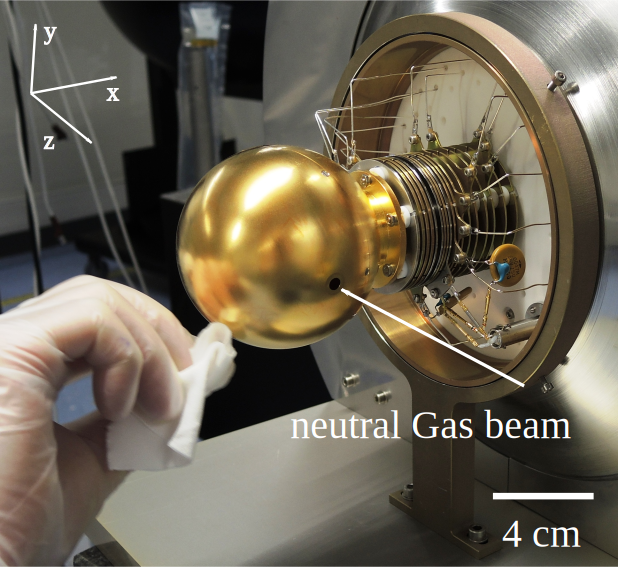
\includegraphics[width = 0.8\textwidth]{Setup/FlightAnte.png}
		\end{subfigure}
		\caption{Left: Prototype antechamber. Right: Flight-like antechamber.}
		\label{fig:SetupAntecham}
	\end{figure}
	\begin{figure}[h] % IS Proto
		\centering
		\includegraphics[width= 0.7\textwidth]{Setup/Proto_IS_sim.png}
		\caption{SIMION Model of the Ion-Source of the NIM Prototype \cite{Diss_Meyer}.}
		\label{fig:SetupProtoISSim}
	\end{figure}
	\begin{figure}[h] % IS PFM
		\centering
		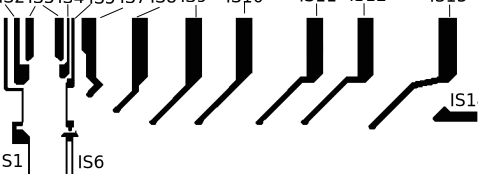
\includegraphics[width=0.7\textwidth]{Setup/ISFlight_bearb.png}
		\caption{SIMION Model of the Ion-Source of the NIM ProtoFlight Model.}
		\label{fig:SetupPFMISSim}
	\end{figure}
	\begin{figure}[h!] % Filament blocs
		\begin{subfigure}{0.5\textwidth}
			\centering
			\includegraphics[width =0.85\textwidth]{Setup/Proto_FilEl_sim.jpg}
		\end{subfigure}
		\begin{subfigure}{0.5\textwidth}
			\centering
			\includegraphics[width = 0.85\textwidth]{Setup/PFM_FilEl_sim.jpg}
		\end{subfigure}
		\caption{Left: Prototype filament housing. Right: PFM filament housing.}
		\label{fig:SetupFilElSim}
	\end{figure}
	This chapter compares the NIM prototype (Fig.~\ref{fig:SetupProto}) with the NIM ProtoFlight Model (PFM) (Fig.~\ref{fig:SetupPFM}) from the mechanical point of view. It shows the key differences between the two models. Special focus lay hereby on the design of the detector because there were made some major design improvements.\\
	Fig.~\ref{fig:SetupAntecham}~left shows the prototype antechamber and right the PFM antechamber. To improve the performance of the antechamber, the flight antechamber was made twice as big as the old one of the prototype. In addition, it has two entrance holes at $\pm$30° relative to the x-axis of the instrument to be able to measure gas coming from both directions of the instrument (see Chap~\ref{subsubsec:Calfly}). The main inflow direction of the neutral particle beam generated by the CASYMIR test facility is 90° \cite{CASYMIR_Graf2004}. Therefore, a second flight-like test antechamber was made which has the second entrance hole at position 90° to be able to test the flight antechamber. The antechambers consists of two parts which are hold together with screws. Tests revealed that two of the mounting screws generate signal artefacts \cite{Meyer_2017_ante}. Therefore, the outer surface of the antechamber was redesigned (see also Chap.~\ref{subsec:ExpAnteCham}).\\
	Fig.~\ref{fig:SetupProtoISSim} shows the SIMION model of the Prototype ion-source, Fig.~\ref{fig:SetupPFMISSim} shows the ion-source of the PFM and Fig.~\ref{fig:SetupFilElSim} shows the filament housing of the Prototype (left) and of the PFM (right). The PFM ion-source has seven electrodes less then the prototype to simplify the source and the flight electronics. Manly LV electrodes were taken together such as IS1\& 2, IS3 \& 4 and IS6 \& 7. IS10 was removed and IS11 was shifted towards the ionisation region. In the filament housing the electron repelling electrodes Fil2--5 were taken together to one single electrode Fil2. The electron repelling electrode in the prototype was split into four parts to compensate with the electric fields for a bad alignment of the filament. For the PFM, the mounting of the filament holder was improved and therefore these four electrodes could be taken together to one single electrode.\\
	Fig.\ref{fig:SetupProtoReflSim} shows a schematics of the ion-mirror. The prototype ion-mirror consists of 14 ring-electrodes (R2--R15). R1 is the drift tube. Between the electrodes R4--R15 are resistors to connect the electrodes with each other to generate a linear voltage gradient when a voltage is applied at electrodes R4 and R15. In addition, a voltage can be applied on electrode R8 allowing additional focusing of the ions in the ion-mirror. The flight ion-mirror consists of a ceramic tube with two resistance spirals on its inner walls replacing electrodes R5--R7 and R9--R14. From the electrical point of view, the two ion-mirrors behave the same.\\
	\begin{figure}[H] % ion mirror
		\centering
		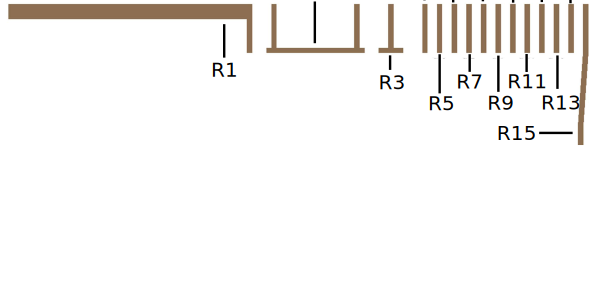
\includegraphics[width=0.9\textwidth]{Setup/Prototype_Reflectron_sim.png}
		\caption{SIMION Model of the ion-mirror of the NIM Prototype \cite{Diss_Meyer}.}
		\label{fig:SetupProtoReflSim}
	\end{figure}
	% Detector Figs.	
	\begin{figure}[H] % Photograph of the Prototype an Flight detector.
		\begin{subfigure}{0.5\textwidth}
			\centering
			\includegraphics[width=\textwidth]{Setup/Prototype_Detector.png}
		\end{subfigure}
		\begin{subfigure}{0.5\textwidth}
			\centering
			\includegraphics[width=.9\textwidth]{Setup/Flight_Detector.png}
		\end{subfigure}
		\caption{Left: NIM Prototype detector \cite{Diss_Meyer}. Right: NIM Flight detector without its radiation shield.}
		\label{fig:DetPhotos}
	\end{figure}
	\begin{figure}[h] % Schematics of the 2 detector designs.
		\centering
		\includegraphics[width= \textwidth]{Setup/PFMDetectors.png}
		\caption{Schematics of the PFM detector housings. Left: preliminary design. Right: final flight design.}
		\label{fig:FlightDetSchemata}
	\end{figure}
	\begin{figure}[h] % Circuit diagram
		\centering
		\includegraphics[width = .8\textwidth]{Bilder/Detector_elec_schema.png}
		\caption{Electrical schematics of the NIM flight detector with laboratory electronics attached.}
		\label{fig:FlighElecSchema}
	\end{figure}
	% free play = technisch Spiel. Put it in during proofreading.
	The NIM Prototype detector has a rigid Printed Circuit Board (PCB) on which the electrical components and the drift tube with the MCP stack are mounted (Fig.~\ref{fig:DetPhotos}~left). Due to Jupiter's strong radiation field, the detector has to be shielded to reduce the noise level induced by the strong radiation and to increase the detector's lifetime. To minimized the required shielding mass, the flight detector has to be very compact. This was achieved by using a flex PCB to fold the detector into a peek housing (Fig.~\ref{fig:DetPhotos}~right). Fig.~\ref{fig:FlightDetSchemata}~left shows the schema of a preliminary design of the peek housing containing the MCPs. The MCPs lay on a ledge 1~mm above the anode. A diode generates a voltage between the MCP backside and the anode to accelerate the electrons from the MCP backside towards the anode (see electrical schema Fig,\,\ref{fig:FlighElecSchema}). There are two contact lugs on top and at the bottom of the MCP stack to apply a voltage over the MCPs. The MCPs are fixed with a peek screw within the housing. In the old design, the screw threads were milled down to the ledge. When the MCPs were mounted, they often canted in the threads. In addition, it was not possible to determine, how much the screw had to be tightened. When the screw was tighten too much, the MCPs broke as they consist of lead glass and are therefore very fragile. When the screw was too loose, the two contact lugs had no reliable contact to the MCPs. When applying a high voltage over the whole MCP stack, the gaps between the contact lugs and the MCPs act as an additional resistors over which the voltage builds up resulting in a discharge between the electrodes and the MCPs. The discharge can propagate through the whole MCP stack and damages the readout electronics. As a consequence, the screw thread was milled less far and an additional mechanical stop was made to tighten the screw only down to that stop (Fig.\,\ref{fig:FlightDetSchemata}~right). This prevented the MCPs from canting in the screw thread thus it was not milled down to the bottom of the lower ledge and with the mechanical stop, the screw could not be tightened too much to break the MCPs. In addition, a peek space was added between the screw and the MCPs to push down the MCPs uniformly. Due to the tolerances in the manufacturing process of the different parts of the housing, metallic spacer rings are added between the peek spacer and the contact lug of the top MCP to close the resulting gap. The number of added rings varies between each detector because the gap is different for each manufactured housing. With this design, the contact between the MCPs and the contact lugs could be improved but from the electrical point of view its still not a clean electrical contact. To make the system more robust against discharges the Zener diode was exchanged through a resistor ($R_D$ in Fig.~\ref{fig:FlighElecSchema}). The flight electronics sets the voltage $U_{stack}$ between the top MCP and the anode. The MCPs and the diode act as resistors, which are connected in series. Therefore, the potential drop over the MCPs depends on the potential drop over the diode. The voltage drop over a Zener diode is 180~V independent of $U_{stack}$. Therefore, the voltage over the MCPs $U_{MCP}$ is 180~V lower than $U_{stack}$. When having a resistor $R_D$ instead of a diode, the voltage over the MCPs cannot be calculated by just having $U_{stack}$ because the resistance of the MCPs $R_{MCP}$ depends on the voltage $U_{MCP}$ applied over them. It also changes with time due to ageing because the conductive material inside the MCP channels degrades over time. Therefore, the current $I_{MCP}$ flowing through the system has to be known to be able to calculate $U_{MCP}$. The NIM flight electronics is not designed to measure this current because it was designed for a detector with a diode where a current measurement would be unnecessary. A calibration with the laboratory electronics was done to determine the relationship between $U_{stack}$ and $U_{MCP}$ (Chap.~\ref{chapExp:Det}).\\
	In the following section, $U_{MCP}$ is derived as a function of the different voltages known when measuring with laboratory electronics. Fig.~\ref{fig:FlighElecSchema} shows the circuit diagram of the detector when operated with laboratory electronics and Table~\ref{tab:ElecSchemaVariableList} summarizes the used variables. The current flowing through the MCPs $I_{MCP}$ is measured with the resistor $R_M$:
	\begin{equation}
		I_{MCP} = \frac{U_{RM}}{R_{M}}
	\end{equation}
	With $U_{RM}$ the voltage over the resistor $R_{M}$ which is:
	\begin{align}
		U_{RM} &= U_{PSA} - U_{A}\\
			   &= U_{PSMCP} + U_{PSD} - U_A
	\end{align}
	With $U_{PSA}$ the power supply output voltage for the anode, $U_{A}$ the voltage applied on the detector anode, $U_{PSD}$ the power supply output voltage applied at the top contact lug of the MCP stack and $U_{PSMCP}$ the voltage difference between the two power supply outputs. $U_{PSMCP}$ is:
	\begin{equation}
		U_{PSMCP} = U_{RM} + 2\cdot U_{Ri} + U_{RD} + U_{MCP}
		\label{eq:UpsmcpTot}
	\end{equation}
	With $U_{Ri}$ the voltage over the input resistors $R_i$, which are there to damp noise coupled into the detector circuit from the power supply:
	\begin{equation}
		U_{Ri} = I_{MCP}\cdot R_i
	\end{equation} 
	$U_{RD}$ is the voltage over the resistor $R_D$ replacing the former diode. The current $I_A$ induced when an ion generates an electron avalanche, is very low compared to the current $I_{RD}$. Therefore, $I_{MCP} = I_{RD}$ and:
	\begin{equation}
		U_{RD} = I_{MCP}\cdot R_D
	\end{equation}
	Solving Eq.~\eqref{eq:UpsmcpTot} to $U_{MCP}$ and inserting the different voltages results in:
	\begin{align}
		U_{MCP} =& U_{PSMCP} - U_{RM} - 2\cdot U_{Ri} - U_{RD}\\
				=& U_{PSMCP} - U_{PSMCP} + U_{PSD} - U_A - 2\cdot I_{MCP} R_i - I_{MCP} R_D\\
				=& (U_A - U_{PSD})\cdot(1 + \frac{2R_i + R_D}{R_M}) - U_{PSMCP}\frac{2R_i + R_D}{R_M}
	\end{align}	
	
	\begin{table}[h]
		\begin{center}
		\begin{tabular}{|m{1.5cm}|m{5.4cm}|m{1.5cm}|m{5.4cm}|}
			\hline
			R\textsubscript{D}& Resistor replacing the former diode & U\textsubscript{A}& Voltage on the detector anode \\
			R\textsubscript{i} & Detector input resistor & U\textsubscript{MCP}& Voltage over the MCPs \\
			R\textsubscript{M}& Resistor used to determine I\textsubscript{MCP} &U\textsubscript{PSA} & Anode voltage output of power supply \\
			R\textsubscript{MCP}& MCP resistance & U\textsubscript{PSD} & Drift voltage output of power supply \\
			R\textsubscript{T} & 50\,$\Omega$ termination & U\textsubscript{PSMCP} & Voltage difference  between U\textsubscript{PSA} and U\textsubscript{PSD} \\
			I\textsubscript{A} & Current induced in the MCPs when an ion hits the MCPs & U\textsubscript{RD}& Voltage over R\textsubscript{D} \\
			I\textsubscript{ion} & Ion current hitting the MCPs & U\textsubscript{Ri}& Voltage over R\textsubscript{i} \\
			I\textsubscript{MCP} & Current flowing through the MCPs &U\textsubscript{RM}& Voltage over test resistor R\textsubscript{M}\\
			I\textsubscript{RD} & Current flowing through R\textsubscript{D} &&\\
			\hline
		\end{tabular}
		\end{center}
		\caption{List of the variables used in the schematics of the flight detector Fig.~\ref{fig:FlighElecSchema} when the detector is operated with laboratory electronics.}
		\label{tab:ElecSchemaVariableList}
	\end{table}
	\begin{figure}[h!]
		\centering
		\includegraphics[width= 0.95\textwidth]{Setup/NIM_schema.pdf}
		\caption{Schematics of the NIM flight design with all electrodes marked in red.}
		\label{fig:MINPFMTot}
	\end{figure}
	\begin{comment}
	% Pumpstand nr.~2 was used to perform stand-alone tests with the different NIM detectors. The test setup consists of a vacuum chamber, a HV power supply, an oscilloscope, a computer to remote control the oscilloscope and a HV meter (Fig.~\ref{fig:Pumpstand2}).		
	
	\begin{figure}[h]
	\begin{subfigure}{.5\textwidth}
	\centering
	\includegraphics[width=0.8\textwidth]{Bilder/Galerie_Setup/Pumpstand2_midres.png}
	\end{subfigure}
	\begin{subfigure}{.5\textwidth}
	\centering
	\includegraphics[width=\textwidth]{Bilder/Galerie_Setup/Pumpstand_PSOszi.png}
	\end{subfigure}
	\caption{Left: Pumpstand nr. 2. Right: Power supply, oscilloscope and control computer for the stand-alone tests of the detector. The signal on the oscilloscope is a noise signal.}
	\label{fig:Pumpstand2}
	\end{figure}
	\end{comment}



	\clearpage
	\newpage
	\thispagestyle{empty}
	\null
	\newpage
	% !TEX root = arbeit.tex
\section{Experiments} \label{sec:Exp}
	The tests described in this chapter include tests of the different components of the NIM instrument such as laboratory tests of the flight antechamber tested on the Prototype or the flight ion-mirror. The part of Chapter \ref{sec:Exp} includes manly test with the prototype, later on tests with the PFM and follow.

% In zeitlicher Reihenfolgen auflisten, damit man sieht, zu welchem Zeitpunkt man mit welchen Teilen gearbeitet hat.
% In this section, all the different test (lab and simulations) are listed. As far as possible in their chronolocial order because between some lab tests there were simulations to improve the instrument before testing the redesigned instrument.

% Fügt ein PDF ein, nummeriert nach dem PDF normal weiter.
%\includepdf[pages=-]{Report_Thermofoil_UV_Masterarbeit.pdf}

% Section über Detector? haben wir ja nicht wirklich etwas gemacht. Diode durch 2 Widerstände ersetzt. -> Spannungsfestigkeit. Verlauf der Überschläge. Unterschiedliche Skizzen.

	In this section, the different tests are described to develop the NIM instrument. Different parts of the instrument were tested to improve the instrument.
%-----------------------------------------------------------------------------------
	\subsection{Ion-Mirror}
	% Test of subcomponents.
	The NIM prototype reflectron was exchanged through the flight like reflectron, which was tested. The NIM prototype reflectron consisted of 12 ring electrodes connected with each other with resistors in between them. On the first, 5th and 12th electrode, a voltage can be applied. With the different resistors, a linear voltage gradient in the reflectron is generated.\\ % Noch besser formulieren.
	The flight reflectron consists of a ceramic tube with two resistance spirals on its inner walls. There are three electrodes, where the voltage can be applied. The electrodes are connected via resistance spirals with each other. The two reflectrons can be seen in Fig.\,\ref{fig:ExpRefl}. This kind of reflectron was also used in the RTOF mass spectrometer which flied in ROSINA \cite{Diss_Scherer} and the in the NGMS \cite{Diss_Hofer}. \\ % Evt. noch etwas schöner und weiter ausführen. Strahlungsfestigkeit musste getestet werden. Report? Paper? Diss?
	Therefore, the two reflectrons are from the electrical point of view the same.\\ % Oder kommt das erst bei der Auswertung?
	
	\begin{figure}[h]
		\begin{subfigure}{0.5\textwidth}
			\centering
			\includegraphics[width = 0.95\textwidth]{Experiments/reflectron_Prototype1.jpg}
		\end{subfigure}
		\begin{subfigure}{0.5\textwidth}
			\centering
			\includegraphics[width = 0.85\textwidth]{Experiments/reflectron_flight.JPG}
		\end{subfigure}
		\caption{Left: Prototype reflectron with ringelectrodes. Right: Flight reflectron}
		\label{fig:ExpRefl}
	\end{figure}

	\subsubsection{Measurement Principle}\label{subsec:ReflecMeasPric}
		% Vortrag Messbedingungen zusammenschreiben
	
	\subsubsection{Discussion}\label{subsec:ReflecDissc}
		% Graphiken neu machen. Achsenskalierung, Spannungssets-Vergleich? Nur sagen, dass sie beinahe identisch sind.
	
	
	% Messbedingungen. Eigenes kurzes Unterkapitel machen
	% Auswertung, eigenes kurzes Unterkapitel

	\begin{comment}
	
	Exchange of the reflectron. Messdaten und Auswertung. Spannungssets vergleichen. Vortrag zusammenschreiben. Plots von dort nehmen und noch etwas besser beschreiben.
	(Plot-Axis, enlarge the exponent of the 10^11 e-/ns)
						
	\end{comment}
	
	
	
	\subsection{Prototype CASYMIR-D/-E}
	% CASYMIR-D? Erst wenn man intensitätsproblem mit ante chamber gelöst hat :/. CASYMIR-E-Kampagne.
	% Kurzfassung?
	
%--------------------------------------------------------------------------------
	\subsection{Simulations}
	
	During development, the mounting of the HV lenses was adapted. Simulations had to be done because as a result of the changed form of the lenses, the voltage set also changed. In this case, the voltage ranges increase by about blabla volts. These new higher ranges challenged the design of the supply electronics because the electronics has a limited amount of space. % Look up the details. Explanation with the electric fields?
	
	%\textcolor{red}{\textbf{Simulations of the adaption of the mounting of the electrodes has to come before the experiments with the PFM although the PFM structure is explained before.}}
	
	% Maybe an other arrangement of the Simulations chaper. See whicht simulations are performed how far any in which order they have to be to be comprehendible.
	
	% Evt. in einem eigenen Kapitel? Schauen, welchen Einfluss es dann jeweis auf die Hardware hatte. -> Elektronik setzt Spannungsranges, beschreiben, dass man da iterieren musste um das optimale Simulationsspannungsset zu finden mit den Grenzen, welche die Elektronik uns für die jeweiligen Elektroden gibt. -> vgl. mit den Messungen vom PFM.
	% Neusimulationen mit neuen Grenzen für die HV. -> die Resultate dieser Simulationen. Als Folgen davon wurden die Grenzen für die HV neu definiert. Schauen, wie man das am besten auseinander nimmt :/.

	% Change of the mounting of the IS lenses -> change in voltages

	% Pulsersimulationen -> Kriterien für Andy für das Pulserdesign. Ab wann wir einen Einbruch in der Massenauflösung haben. (Worddokument wo die einzelnen Bilder zusammengestellt sind?)
	
	% Filament repeller simulation tests. Noch Graphiken einmal einfügen. Die wichtigsten.
	% Um herauszufinden, wie wichtig die Position des Filaments ist.
	
	% Noch besser umschreiben. Die position des filaments entspricht nicht der erwarteten??? Was ist da schief gelaufen??? :(
	
	% Intensitätssimulation Countberechnung:
	% Man generiert 2000 e- auf dem Filament und zeichnet immer nach 1E-5 microsec auf, an welcher Position sich die Teilchen gerade befinden. Die Fkt. 'Plot_optVoltAndPos.m' zählt alle Positionen zusammen, welche sich in dem Zylindervolumen befinden. Die Grundfläche des Zylinders ist das Eintritts-Grid von der antechamber und die Höhe ist die Höhe der Entrance. Im th-Mode befinden sich nur in diesem Volumen neutrale Teilchen.
	\begin{figure}[h]
		\begin{subfigure}{0.53\textwidth}
			\centering
			\includegraphics[width= 0.95\textwidth]{Experiments/SimRepPosU.png}
		\end{subfigure}
		\begin{subfigure}{0.47\textwidth}
			\centering
			\includegraphics[width= 0.95\textwidth]{Experiments/SimRepPosImax.png}
		\end{subfigure}
		\caption{Left: The filament repeller voltage to reach the maximum electron intensity over the volume of the neutral particles. Right: Electron intensity normed on the intensity at position 0.} % Noch Graphik wie Intensität bei den versch. Pos abfällt.
		\label{fig:ExpSimRep}
	\end{figure}

	\subsection{Filament decision}
	% Ranking criterion -> Explanation, see electronics book. constant power of one filament -> resistance variies over time. Vgl. Diss Rico.

%------------------------------------------------------------------------------------
	\subsection{Pulser}
	% Simulations with different rise times and their influence on the mass spectrum.
	% Test with lab pulser, wavelab pulser -> compare their properties and their performance.
	
	% Pulsertests, Messungen, Simulationsresultate
	% Two different pulsers properties, pulse shape. Tests with different gases. Massresolution, Intensity relation?, SNR? Are these two properties correlated? Noch mit Peter anschauen. Ar sieht in allen 4 Fällen etwas komisch aus. Higher signal intensity -> higher SNR.
	% Achsenskalierung anschauen von Areagraphik. Wenn das geklärt ist, evt. in Matlab schreiben. Zusätzliches Skript für diese Graphiken, Stefans Vorlagen anschauen. Die signal intensity lässt sich nicht einfach in Druck umrechnen. Zu viele unbekannte Komponenten -> a.u. oder # e-/ns angeben.
	
	
	
	\subsection{Detector Tests}
	% FS IsoArea. Variation of the MCP gain an observation how the SNR and IsoArea change. \\titania.unibe.ch\UserHomes\foehn\MyDocuments\PhD\Messungen\FS\ firstOpti\MCP_Gain.opj
	% Also show different signal heights/ forms? Defect diode, functioning diode, resistor? Full gain curve is only possible for functioning diode (tests to be done) and resistor (plot already included).
	The following chapter describes improvements of the mechanical and electrical design of the NIM PFM detector and tests performed with different versions. Most of the tests were performed in the Pumpstand nr.2 (Chapter \ref{subsubsec:SetFacPumpst}) and a few were done with the detector in the sensor Proto Flight Model (PFM) or in the sensor flight spare model (FS).\\
	% Leave this part here as it is a description of the process we were working on. Describe the adaption of the meachanical design of the detector housing, the consequence that we inserted a resistor instead of an anode. Pros and Cons of the Anode vs. the resistor?
	% Description of the housing and problems related to it -> investigation, improvements.
	The detector suffered repeatedly discharges causing a failure of the diode, which is one of the key components of the detector. This lead to a redesign of the detector housing and to an exchange of the diode through a resistor, because the resistor is more robust concerning discharges. % Include an electrical schema. May a zoom of the other one laready included in the setup chapter (as soon as it is finished). Explanation about how a diode works? Talk with JoGa maybe. Explain main hypothesis why it died repeatedly?
	The discharges could be eliminated by a redesign of the detector housing. % Vgl. Fig. of the 2 housing designs (start and end) and explain them.
	Fig.bla left shows an earlier version of the detector housing and Fig. bla right shows the design of the current flight detector.
	Basically, the MCPs lay on a border about 1 mm above the anode. % Check distance
	A diode generates an additional voltage difference between the MCP backside and the anode to accelerate the electrons from the MCP backside towards the anode. Between this border and the MCP is the contact lug which is connected to the high voltage rail. On top of the upper MCP is the contact lug to connected to the corresponding voltage rail. On top of that is a bushing and a sort of screw. When tightening the screw, the bushing presses uniformly on the MCPs. In the old design, the thread for the screw was cut down to the boarder on which the MCPs lay. When assembling the whole stack, the MCPs often cant in the thread. Another challenge lay in tightening of the screw. When the screw was too loose, the top and the bottom contact lug had no reliable contact to the MCPs. When applying a high voltage over the whole MCP stack, the gap acts as an additional resistor over which the voltage build up resulting in a discharge between the corresponding electrode and the MCP. The discharge can propagate through the whole MCP stack and damage the diode and the capacitors. When the screw was tighten too much, the MCPs broke as they consist of lead glass and are very delicate in the mechanical point of view. As a consequence, the screw thread was cut less deep down and an additional boarder was made on which the bushing was pressed by the screw to make the assembly of the detector easier. In addition, the diode was exchanged through a resistor because the resistor is more robust in regards to the discharges. Due to the uncertainty in the manufacturing process of the detector housing, spacer rings are added between the bushing and the MCP to really close the gap. Due to that uncertainty, the number of rings needed for each detector has to be determined by trial.
	% Insert a Figure of the housing. Further explanation of the design
	% free play = thechnisch für Spiel
	% Circuit diagram with both options diode and resistor. Ref for that statement?
	% Upgrade SNp6.
	
	% Explanation of the different meas Figs.
	% Detector with broken anode is detector EM4. Look if there are any specifications. Seems to have most probable the same configuration as the other detectors. -> Sufficient for the data analysis but it would be good to have the datasheet.
	Fig. bla shows the signal shapes of different detector configurations beginning with the shape of a detector with a broken diode. The other two figures show the signal shape of a detector with a functioning diode and a functioning resistor. The most remarkable feature is that the signal height of the detector is much smaller and much broader that the signal shape of the other two configurations. In addition, the first overshoot is much lager due to the impedance mismatch caused by the broken diode. A broken diode gets conductive and therefore the potential at the MCP backside is equal to the potential of the anode. The electrons are not additionally accelerated and therefore the resulting signal is smaller than the signal with a functioning diode.\\
	Fig.\ref{fig:SN4p54p7Gain} shows the gain curves of two potential FS detectors both in the configuration with a 10\,\si{\mega\ohm} resistor instead of a diode. 
	% Other parameters to analyse? Pulse width of the 3 configurations? Overshoot? Can that really be calculated out of the data? Impedance match based on the overshoot.
	\begin{figure}
		\begin{subfigure}{.5\textwidth}
			\centering
			\includegraphics[width=0.9\textwidth]{Bilder/Gain_Curves_SN4p5_4p7.png}
		\end{subfigure}
		\begin{subfigure}{.5\textwidth}
			\centering
			\includegraphics[width=0.9\textwidth]{Bilder/SN4p7_discharge.png}
		\end{subfigure}
		\caption{Left: Gain curves of two NIM PFM detectors. The difference in gain is because for each measurement curve, a different set of MCPs was used. Right: Gain curves of a folded NIM PFM detector. The lower gain curve was recorded after a discharge at an MCP voltage of 1.8\si{\kilo\volt}.}
		\label{fig:SN4p54p7Gain}
	\end{figure}
	% Discussion about the discharge behaviour in regards to gain. Are there any values? Something with free electrons destroying the inner coating of the MCP channels. Only a rough estimate needed.
	% Explanation of the fit model in theory part. -> Maike if there is any theory about that topic specifically.	
	
	% ROSETTA? When was a resistor latest used? Have a look if there is a space for sort of improvements of the sensor. If it is part of the experiments of of the thery part...
	% Explain, which measurements were made with which MCPs, describe how the discharge influences the signal. How much of the signal we loose in this specific measurement. Literature references?
	% Description of the current measurement of the detector with the laboratory electronics attached and then the calculation of the MCP voltage. State clearly under with circumstances the calculation with this method is possible and under which it is not (ion current, which is falsely taken into account)
	% Precise can we estimate the numbr of ions/ the partial pressure of the gas?
	% Describe, how far we tried to approximate the voltage.
	
	% Plot off the gain curves of the detector in its different states. flat, folded, folded in the wolfram copper shealding.
	% Measuring settings. Turn the drift voltage up to -2.5 kV and then slowly increase the anode voltage to the value you want to measure. The gain is calculated with the software by doing a Simpson 3/8 integration of the peak = Q. (Look in the lab book for the proper calculation)
	% Maybe there is time to redo the tests with the real PFM detector (XD wär schön. Leider nein). (Die Resultate sind nicht so vollständig wie die von der einen anderen Messung. Messung mit einem Zwillingsdetektor und von diesem auf den Flugdetektor schliessen. -> evt. schöne Graphik).
	
	
%-----------------------------------------------------------------------------------
	\subsection{Ionoptics}
	\subsubsection{Voltage Optimisation}
	Two types of electrical lenses. positive and negative voltage lenses. positive and negative voltage lenses have the same effect. In negative voltage lenses, the particles fly faster = shorter time-of-flight. This results in a better mass resolution.\\
	Aim in the lab is to get two different voltage sets. One for positive voltages to not stress the equipment and one with negative voltage lenses to reach the maximal performance of the instrument. -> Tests showed no significant better mass resolution. A more detailed data analysis has to be made. % data in folder: \\titania\UserHomes\foehn\My Documents\PhD\Messungen\PFM\CASYMIR-C\nMode_voltageSet_Comparison_200430 
	
	\subsection{Instrument performance tests}
		% At the end, make a comparison of the discussion of the different instruments as mass resolution, SNR as far as possible.
		\subsubsection{Prototype} % Final results. Only shpw best mass resolution achieved. May revere to Stefan's Diss. With the Prototype there were mainly componenets tests. Only discussion of the antechamber performance if it is not discussed in the chapter above.
		\subsubsection{PFM} % Include here the paper because it give a very good overview over the results conducted with it.
		\subsubsection{FS} % Include here the final results of the FS of this year with lab and flight electronics. Discussion about that subject, see PFM paper.
		% Laboratory and flight electronics are part of the same chapter because with the fligh electronics the only thing worth to discuss is the mass resolution because the signal intensity is still very low. Discuss the SNR graphics with Peter and then finalize this part of the chapter.
		
		% Look up the conditions for the description.
		\textbf{Ion Storage two different velocities}\\ % Ref. to Abplanalp paper.
		Ion storage is very crucial for a time of flight mass spectrometer because every ion generated and not stored in the ion source is lost and can generate additional electrical noise on the detector signal line. In this test the ion storage behaviour of the ion source was analysed for thermal and neutral mode for hydrogen and krypton with velocities of 2\,\si{\kilo\meter\per\second} and 4\,\si{\kilo\meter\per\second}. The emission current was varied from 20 to 600\,\si{\micro\ampere}. Ion storage of positive ions in x- and y- direction is supported by the negative potential generated by the electron beam. Two ring electrodes with a positive voltage applied generate a positive potential ring to trap generated ions in y- and z- direction (Fig.\ref{fig:ExpFSFlightSenIonStorIS}). For emission currents from 20 to 600\,\si{\micro\ampere} according to Eq.\,\eqref{eq:elPotIem} the negative potential in the centre of the electron beam is -0.08-(-2.59)\,\si{\volt}. Fig.\ref{fig:ExpFSFlightSenIonStor} left shows the ion storage behaviour of the ion source of hydrogen and right the ion storage behaviour of krypton. In case of no ion storage, the relationship between the electron emission current I\textsubscript{em} and the signal intensity is linear. In case of ion storage there is a quadratic relationship between I\textsubscript{em} and the signal intensity. When measuring with the thermal mode, the particles get slowed down until they have energies in the range of 0.01\,\si{\electronvolt} and are therefore easy to trap in the potential field. In neutral mode particles enter the ionisation region directly. The kinetic energy of hydrogen for velocities between 2-4\,\si{\kilo\metre\per\sec} is 0.07-0.27\,\si{\electronvolt}. It can therefore easy be trapped in the potential field by the electron beam and the potential of the ring electrode already with very emission currents as low as 20\,\si{\micro\ampere}.\\
		The kinetic energy of \textsuperscript{84}Kr for the same velocities is 2.8-11.2\,\si{\electronvolt}. This energy exceeds the potential of the centre of the electron beam and the ions are therefore more difficult to trap with only the electron beam. The ions are kept in the middle of the ionisation region with the positive potential ring. According to Fig.\,\ref{fig:ExpFSFlightSenIonStor} ion storage for \textsuperscript{84}Kr starts to dominate at emission currents of 100\,\si{\micro\ampere}.
		%Therefore there is no difference in the measured intensities for hydrogen when it enters with 2 or 4\,\si{\kilo\meter\per\second}.\\		
		In thermal mode, an increase in beam velocity leads to an increase in signal intensity due to the density enhancement effect \textcolor{red}{(Ref.)}. Therefore a higher signal intensity is expected in thermal mode for 4\,\si{\kilo\meter\per\second} compared to 2\,\si{\kilo\meter\per\second}. 
		Like the in PFM, the FS shows a nice ion storage behaviour. For krypton ion storage just starts at an emission current of 100\,\si{\micro\ampere} where hydrogen is stored already at lower emission currents due its lower kinetic energy at the same beam velocity.
		
		\begin{figure}[h]
			\centering
			\includegraphics[width = 0.8\textwidth]{Experiments/FiL_IS_elBeam_Storage.png}
			\caption{Ion storage source with sample voltage set applied to the electrodes. In light blue are the potential lines and in dark blue a simulated electron beam.}
			\label{fig:ExpFSFlightSenIonStorIS}
		\end{figure}
		
		
		\begin{figure}[h] % Ion storage. Exchange Graphics as soon as discussed with Peter how to proper show the results.
			\begin{subfigure}{0.5\textwidth}
				\centering
				\includegraphics[width = \textwidth]{Experiments/FSLabIonStorageH2.png}
			\end{subfigure}
			\begin{subfigure}{0.5\textwidth}
				\centering
				\includegraphics[width = \textwidth]{Experiments/FSLabIonStorageKr84.png}
			\end{subfigure}
			\caption{Ion storage measurement with the flight spare sensor but with laboratory electronics attached for H$_2$ and $^{84}$Kr for two different gas velocities.}
			\label{fig:ExpFSFlightSenIonStor}
		\end{figure}

		% Detector behaviour test in FS sensor. Formula derivation is in the theory part with the proper detrivation.
		% No saturation observed. 

		\textbf{Mass resolution and Signal-to-Noise Ratio}\\
		According to the requirements stated in (Ref.) % See paper
		the required mass resolution for neutral mode is 500 and for thermal mode it is 1000 m/dm but to be able to distinguish between different masses at unit masses of 1000\,u NIM has to have a mass resolution of 1000. Otherwise NIM the different unit masses cannot be distinguished. Fig.\,\ref{fig:ExpFSFlightSenMassRes} show two spectra recorded with the NIM flight sensor with laboratory electronics attached with an electron emission current of 100\,\si{\micro\ampere}. With a mass resolution of 708 for neutral gas mode NIM fulfils the requirements. In thermal gas mode the highest mass resolution achieved was 830 m/$\Delta$m which comes close to the requirements. Fig.\,\ref{fig:ExpFSFlightElMassRes} show the mass spectra recorded with the NIM flight sensor with the flight electronics attached. The electron emission current was 200\,\si{\micro\ampere} the highest mass resolution achieved at the current state is 490 m/$\Delta$m for neutral gas mode and 462 m/$\Delta$m for thermal mode. Fig.\,\ref{fig:ExpFSFlightElK78} shows a mass spectrum recorded in thermal mode with an emission current of 300\,\si{\micro\ampere} the $^{78}$Kr peak is clearly visible. The signal to noise ratio for the spectra recorded with the flight electronics is very low compared to the SNR for the spectra recorded with the laboratory electronics. We also observe noisy part wandering between the single spectra. There is a significant part of repetitive noise appearing not always at the same position in the spectrum. With a proper noise filter this noise can be detected and significantly reduced without affecting the mass signal peaks. For future work, there is a lot of potential for improving the spectrum by proper analysing the noise and writing filters to suppress the noise.\\
		Fig.\,\ref{fig:ExpFSFlightSenSNR} shows a mass spectrum recorded with the flight sensor with the laboratory electronics attached. The highest SNR achieved was $6\cdot10^{5}$ and therefore almost 6 decades. % Explanation why the 6 decades are required.
		The mass peaks 355\,u, 390\,u and 429\,u are some oil components with water adducts coming from the used turbo pumps of the test facility. 415\,u is an artefact coming from the background subtraction algorithm. The artefact peak is also wider then the other surrounding mass peaks.
		
		\begin{figure}[h]
			\begin{subfigure}{0.5\textwidth}
				\centering
				\includegraphics[width = \textwidth]{Experiments/FSLabthMode.png}
			\end{subfigure}
			\begin{subfigure}{0.5\textwidth}
				\centering
				\includegraphics[width = \textwidth]{Experiments/FSLabnMode.png}
			\end{subfigure}
			\caption{Mass spectra measured with the flight spare sensor with the laboratory electronics electronics attached. Left: with thermal gas mode Right: neutral mode.}
			\label{fig:ExpFSFlightSenMassRes}
		\end{figure}

		% Mark the noisy part for better description to explain that
		% conditions: nMode UMCP: 1950 V. P = 1.03e-8 mbar 20H2:1Kr
		%			thMode UMCP = 1950 V. P = 6.05e-8 mbar
		\begin{figure}[h]
			\begin{subfigure}{0.5\textwidth}
				\centering
				\includegraphics[width = \textwidth]{Experiments/FSthMode200uA.png}
			\end{subfigure}
			\begin{subfigure}{0.5\textwidth}
				\centering
				\includegraphics[width = \textwidth]{Experiments/FSnMode200uA.png}
			\end{subfigure}
			\caption{Mass spectra measured with the flight spare instrument with the flight electronics attached. Filament emission current was 200 \si{\micro\ampere}. Left: with thermal gas mode Right: neutral mode.}
			\label{fig:ExpFSFlightElMassRes}
		\end{figure}
		
		\begin{figure} % Point out at that picture that the Kr 78 isotope is clearly visible.
			\centering
			\includegraphics[width = 0.6\textwidth]{Experiments/FS_thMode300uA.png}
			\caption{Mass spectra measured with the flight spare instrument with the flight electronics attached. Filament emission current was 300 \si{\micro\ampere}.}
			\label{fig:ExpFSFlightElK78}
		\end{figure}
		
		% SNR 600 uA emission current. Rest gas Ptot = 1.6e-9 mbar, UMCPeff = 1.8 kV. Name the gas peaks. Peaks around 200 u are not mercury because the isotopic ratio does not match the pattern.
		\begin{figure}[h]
			\centering
			\includegraphics[width = 0.7\textwidth]{Experiments/FSLabSNRRestGasPressCal.png}
			\caption{SNR plot for the flight spare sensor but with laboratory electronics attached at a chamber pressure of 1.5$\cdot10^{-9}$\si{\milli\bar}.}
			\label{fig:ExpFSFlightSenSNR}
		\end{figure}
	
	
	
	
	
	
	
	\clearpage
%	% !TEX root = arbeit.tex
\section{Conclusion}

	% Wichtigste Punkte nocheinmal zusammenfassen (Prototyp tests und PFM/ FS tests)
	% Put the final version of the PFM/ FS instrument into this chapter with all the components, Antechamber version, IS... as a summary of the instrument at its final state as it is at the end of the thesis. Just as a short state description.
%	\newpage
%	\thispagestyle{empty}
%	\null
%	\newpage
	% !TEX root = arbeit.tex
\section{Summary and Outlook}
	
	At the beginning of a space mission, there stands always a main scientific question. In case of JUICE its to investigate Jupiter and its icy moons as a planetary system potentially harbouring life. To answer that question, the question is divided into much more concrete questions out of which specific requirements for instruments participating in the space mission result. For the specific case of the NIM instrument, these requirements are the needed mass resolution, the signal-to-noise ratio and the mass range NIM has to detect to determine the composition of the icy moons' exosphere with enough accuracy to set further constraints for exosphere modellers to understand the formation and evolution processes involved to form the icy moons.\\
	The task of a scientist designing and building such an instrument is to identify the needed technical performance of the subsystems of the specific instrument based on the scientific requirements on the instrument performance mentioned above. Examples of such technical requirements are the range and stability of needed voltages to operate the instrument, switching times or gain. Other requirements arise from operations, e.g., the flyby trajectory and orientation of the spacecraft to the subject, which has to be investigated during the mission.\\
	In the following, two examples are shown on which the iteration processes of improving the instrument is shown. On the example of the high-voltage pulse generator it is shown, how important it is to push the operating electronics to their limit to reach higher performance with the new instruments leading to better data and an improvement of our knowledge. The second example focuses on the flyby trajectory and the restrictions arising for the instrument design from the mission itself.\\
	
	Two of the most important parameters of the high-voltage pulse generator used to extract the ions from NIM's ionisation region are the fall time and the bias voltage. The fall time has to be as short as possible to ensure that all ions get the same amount of energy. Otherwise, the mass resolution of especially low mass ions suffers (see Chap.~\ref{chap:massRes}). Typical fall times are in the range of a few ns and theory shows that this is a very critical parameter. Two different flight designs of the high voltage pulse generator were tested during the thesis using the prototype ion-optical system. The tests showed a clear preference to the one with the shorter fall time in agreement with the theory (see \cite{Lasi_IEEE2020}). Another important parameter is the bias voltage, which is the voltage applied on the extraction grid when no high voltage pulse is applied. As shown in Chap.~\ref{chap:FSCalib} and \cite{Foehn2021}, the PFM and FS ion-optical systems have both a good ion storage capability when operated with laboratory electronics. To achieve that it is necessary to have a stable potential well in the ionisation region during the time when no extraction pulse is applied on the extraction grid. This requires that the voltages applied on the electrodes in the ionisation region do not fluctuate more than 100~mV. Laboratory tests showed that the most critical ones with respect to ion storage are the bias voltage applied on the extraction grid and the voltage applied on the grid opposite of the extraction grid. The flight pulse generator shows less good performance with regards to that parameter than the laboratory electronics (see Chap.~\ref{chap:ExpPulser}). Due to other restrictions like the necessary radiation hardness of the electrical components limiting the number of options for certain components, this design was the best with the available resources.\\
	Other requirements appear from the trajectory of the spacecraft. JUICE contains several different instruments. The orientation of the spacecraft depends on the instruments to enable them an optimal FoV on their target. For a spacecraft having solar panels for power generation, it is important for the solar panels to be oriented perpendicular to the Sun whenever possible to optimize power generation especially for missions with targets such far away from the Sun as the mission JUICE with target Jupiter, which introduces constraints on the spacecraft orientation. The second priority for the spacecraft orientation is that the camera has the best view of the observation target on the moons' surface.\\
	For the NIM instrument in particular that meant to have a design with a big FoV to have a certain flexibility regarding the gas inflow direction into the instrument. NIM has an open-source and a closed-source entrance to measure neutral particles and ions directly and to thermalise neutral particles with the closed source antechamber to make advantage of the density enhancement behaviour to amplify the signal with that mode. Simulations of the trajectory of the spacecraft revealed that two entrance holes on the antechamber were necessary to be able to measure during the different flybys even though a second entrance hole leads to a lower performance of the closed-source antechamber (Chap.~\ref{subsubsec:Densenhan} and \ref{subsubsec:Calfly}).\\
	
	The NIM PFM was successfully delivered to the JUICE spacecraft in December 2020 and at the current state, the NIM FS model waits until the JUICE spacecraft started its journey to Jupiter in September 2022. Until then, the FS waits as it is the spare model for the case that something happens to the PFM on the spacecraft until launch. After the start of the spacecraft, the NIM FS has to be properly calibrated with the actual flight electronics. Most results presented in this thesis were conducted with laboratory electronics attached to the two ion-optical systems because there was only very little time to test the whole system. The NIM ion-optical system was first qualified as a separate unit and now there follows the calibration of the whole NIM instrument.\\
	In addition, the flight software is still under development and has to be tested with the full system. The optimiser to optimised the voltage sets during the flight is still under development. As soon as it is available for tests, it has to be tested and the target function used to improve the voltage sets has to be adapted for NIM. First results of the FS ion-optical system operated with flight electronics revealed that there lies a lot of potential in the postprocessing of the data especially in regards to filtering. Therefore a proper filter has to be written to improve the SNR of the final spectra.\\
	To have a proper calibration facility for the NIM instrument and future TOF instruments, the SATANS test facility (Supersonic cATion and ANion Source) is under development to generate neutral particle and ion beams with velocities from 1--15~km/s. The CASYMIR test facility is only able to generate neutral particle beams with velocities up to 4~km/s but the NIM instrument has to detect neutral particles and ions with velocities up to 8~km/s. Therefore, SATANS was developed to have a facility covering a higher velocity range for neutral particles and also for ions. Such a calibration facility in necessary to calibrate the FS instrument and to replicate the data recorded with the actual flight instrument on the satellite to understand the measured data. Therefore, a test setup is required able to reproduce the environment is space as close as possible. First tests performed with the NIM prototype on SATANS showed promising results \cite{SATANS_Meyer2018} but there is still a lot of potential in improving the performance and stability of SATANS. At the current state, SATANS is able to produce an ion beam with velocities between 1~--~15~km/s. As soon as the stability of the ion beam is improved, the system will be upgraded with a neutraliser to also produce a neutral particle beam in this energy range.
	
	
	
	
	
	
	
	
	
	
	
	
	
	
	
	
	
	
	
	\clearpage
	\bibliography{Quellen}
	\clearpage
	% !TEX root = arbeit.tex
\section{Appendix} \label{sec:appendix}

	% Schauen, was da alles reinkommt.
	% Startup Procedure of both filaments.
	\clearpage
	
	\section*{Acknowledgement}
	
	% More details.
	My thanks go to:
	
	Prof. Dr. Peter Wurz for the opportunity to work on the NIM instrument giving me a very good insight on how such projects work. The work was very instructive from the physical and the technical point of view. I also appreciated the educational discussions.
%	Enduring my shenanigans.
	
	Stefan Meyer who introduced me to the NIM instrument and made me familiar with all the other teams members.
		
	Harald Mischler and the team from the mechanic's workshop of the University of Bern and also to my office colleagues Georg Bodmer, Adrian Etter and Joël Gonseth for their technical support in the laboratory and the amusing discussions in our office.

	Daniele Piazza, Michael Gerber and Stefan Brüngger from the mechanical construction.
	
	Matthias Lüthi, Severin Oegschger, Andreas Nentwig, Michael Althaus, Philipp Fahrer and Hans~Peter Munz for the electronics workshop.
	
	André Galli as an office mate and also for the very stimulating discussions especially during the time writing this thesis.
	
	The Wabschli-WG namely Marc Trautmann, Jonathan Gasser, Viviane Tanner and Sabrina Waldburger.
	
	My family
	
	The members of the Dinner's club, the Friday beer and the Alpweeked. Especially Lukas Jaun.

	Colleagues at the institute for their
	
	\newpage
	\thispagestyle{empty}
	\null
	\newpage
	
	\includepdf[pages=-]{MSc_Masterarbeit_erklaerung.pdf}
	
\end{document}




